%\pdfminorversion=7 %added to avoid warning about pdf versions
%note Non-PDF special ignored! warning may be related to the .cls using ps commands somewhere.
%\documentclass[12pt,letterpaper,fleqn]{article}


%%%%%%%%%%%BEGIN MBE Commands %%%%%%%%%%%%
\documentclass[onecolumn,fleqn,nogrid]{MBE}%


\usepackage{url}

\jshort{mbe}

\volname{}

\jvolume{0}

\jvol{}

\jissue{0}

\pubyear{2018}

\mstype{Article}

\artid{XXX}

\access{Version Posted on BioRXiV on June 6, 2018}



%%%END MBE COMMANDS

%%Older packages
%\usepackage[english]{babel}
\usepackage[normalem]{ulem}
\usepackage{bm} %provides more obvious bold versions o greek glyphs
\usepackage{amsfonts}
\usepackage{amsmath}
\usepackage{amssymb}
\usepackage{amstext}
\usepackage{amsthm}
\usepackage{array}
%\usepackage{booktabs}
%\usepackage{caption}
\usepackage{color}
%\usepackage{epsfig}
%\usepackage{fixltx2e} %unneeded after 2015
\usepackage{float}
%\usepackage{fullpage}
%\usepackage{nameref}
%\usepackage{hyperref} %also provides \nameref
\usepackage{ifthen}
\usepackage{indentfirst}
\usepackage{latexsym}
\usepackage{longtable}
%\usepackage{lscape}
%\usepackage{mhchem}
%\usepackage{natbib}
%\usepackage{pifont}
%\usepackage{setspace}
%\usepackage{textcomp}
%\usepackage{verbatim}
\usepackage{fancyhdr}
\usepackage{graphicx}

\usepackage{ifdraft}
\ifdraft{\renewcommand{\includegraphics}[2][]{\\}

}{\relax}

%\pagestyle{headings}


%%%%%%%%%%%END SYS BIO COMMANDS %%%%%%%%%%%%


%\usepackage[doublespacing]{setspace}
%\usepackage[nomarkers,figuresonly]{endfloat}  %%place all figures at end
%\usepackage{amsmath, amssymb,amsfonts}
%\usepackage{fullpage} %this causes problems with the sysbio style file
%\usepackage[normalem]{ulem} %strike out via \sout{}
%\usepackage[small]{caption}
\usepackage{datetime} %provides \currenttime command



%\usepackage{subfig}

\usepackage{xspace}

%%modified from MBE.cls
%\usepackage[mathlines,switch,modulo,pagewise]{lineno}%\pagewiselinenumbers[switch]
%\modulolinenumbers[2]

\usepackage{lineno}
\linenumbers
%\modulolinenumbers[2]


%%Fix issue with lineno and math environment
%% Taken from https://tex.stackexchange.com/a/55297
\newcommand*\patchAmsMathEnvironmentForLineno[1]{%
  \expandafter\let\csname old#1\expandafter\endcsname\csname #1\endcsname
  \expandafter\let\csname oldend#1\expandafter\endcsname\csname end#1\endcsname
  \renewenvironment{#1}%
     {\linenomath\csname old#1\endcsname}%
     {\csname oldend#1\endcsname\endlinenomath}}%
\newcommand*\patchBothAmsMathEnvironmentsForLineno[1]{%
  \patchAmsMathEnvironmentForLineno{#1}%
  \patchAmsMathEnvironmentForLineno{#1*}}%
\AtBeginDocument{%
\patchBothAmsMathEnvironmentsForLineno{equation}%
\patchBothAmsMathEnvironmentsForLineno{align}%
\patchBothAmsMathEnvironmentsForLineno{flalign}%
\patchBothAmsMathEnvironmentsForLineno{alignat}%
\patchBothAmsMathEnvironmentsForLineno{gather}%
\patchBothAmsMathEnvironmentsForLineno{multline}%
}


\graphicspath{{./Figures/}} \DeclareGraphicsExtensions{.pdf, .jpg, .png}

%reduce font size of margin paragraphs \marginpar
\makeatletter
\long\def\@ympar#1{%
  \@savemarbox\@marbox{\tiny #1}%
  \global\setbox\@currbox\copy\@marbox
  \@xympar}
\makeatother

%%%%%%%%%%%%%%%%%%%%%%%%%%%%%%%%%Local Commands%%%%%%%%%%%%%%%%%%%%%%%%%%%%%
%%% Sort using M-x 'sort-lines'
\newcommand{\PC}{physicochemical\xspace}
\newcommand{\Costaobsvec}{\ensuremath{\Cost(\aobsvec)}\xspace}
\newcommand{\Costaveci}{\ensuremath{\Cost(\aveci)}\xspace}
\newcommand{\Costavecj}{\ensuremath{\Cost(\avecj)}\xspace}
\newcommand{\Costavec}{\ensuremath{\Cost(\avec)}\xspace}
\newcommand{\Costcveci}{\ensuremath{\Cost(\cveci)}\xspace}
\newcommand{\Costcvecj}{\ensuremath{\Cost(\cvecj)}\xspace}
\newcommand{\Cost}{\ensuremath{\text{\textbf{C}}}\xspace}
\newcommand{\DeltaAIC}{\ensuremath{\Delta\text{AIC}}\xspace}
\newcommand{\DeltaAICc}{\ensuremath{\Delta\text{AICc}}\xspace}
\newcommand{\AICw}{\ensuremath{\text{AIC}_\text{w}}\xspace}
\newcommand{\EE}{\mathbb{E}} %use for expectation function E()
\newcommand{\Funcaobsvec}{\ensuremath{\Func(\aobsvec|\aoptvec)}\xspace}
\newcommand{\Funcaoptvec}{\ensuremath{\Func(\aoptvec|\aoptvec)}\xspace}
\newcommand{\Funcaveci}{\ensuremath{\Func(\aveci|\aoptvec)}\xspace}
\newcommand{\Funcavecj}{\ensuremath{\Func(\avecj|\aoptvec)}\xspace}
\newcommand{\Funcavec}{\ensuremath{\Func(\avec|\aoptvec)}\xspace}
\newcommand{\Funccveci}{\ensuremath{\Func(\cveci|\aoptvec)}\xspace}
\newcommand{\Funccvec}{\ensuremath{\Func(\cvec|\aoptvec)}\xspace}
\newcommand{\Func}{\ensuremath{\text{\textbf{B}}}\xspace}
\newcommand{\GTR}{GTR+$\Gamma$\xspace}
\newcommand{\LogN}{\ensuremath{\text{LogN}}\xspace}
\newcommand{\Ne}{\ensuremath{{N_e}}\xspace} %
\newcommand{\Nemu}{\ensuremath{{N_e \mu}}\xspace} %
\newcommand{\Lik}{\ensuremath{\mathcal{L}}\xspace}%replaces \Lmatrix which was inconsistent and, thus, confusing
\newcommand{\pimatrix}{\ensuremath{\boldsymbol{\pi}}\xspace}
\newcommand{\mumatrix}{\ensuremath{\boldsymbol{\mu}}\xspace}
\newcommand{\Pmatrix}{\ensuremath{\mathbf{P}}\xspace}
\newcommand{\Tmatrix}{\ensuremath{\mathbf{T}}\xspace}
\newcommand{\Dmatrix}{\ensuremath{\mathbf{D}}\xspace}
\newcommand{\Dmatrixp}{\ensuremath{\mathbf{D}_p}\xspace}
\newcommand{\Mmatrix}{\ensuremath{\mathbf{M}}\xspace}
\newcommand{\Qmatrix}{\ensuremath{\mathbf{Q}}\xspace}
\newcommand{\Qmatrixa}{\ensuremath{\Qmatrix_a}\xspace}
\newcommand{\Wi}{\ensuremath{{W_i}}\xspace}
\newcommand{\Wj}{\ensuremath{{W_j}}\xspace}
\newcommand{\simP}{\ensuremath{\sim P}\xspace}
\newcommand{\selac}{SelAC\xspace}
\newcommand{\selacplusgamma}{SelAC$+\Gamma$\xspace}
\newcommand{\selacmaj}{SelAC$_{M}$\xspace}
\newcommand{\selacmajplusgamma}{SelAC$_{M}+\Gamma$\xspace}
\newcommand{\acivec}{\ensuremath{a\left(\cveci\right)}\xspace}
\newcommand{\acvecg}{\ensuremath{a\left(\vec{c}_{i,g}\right)}\xspace}
\newcommand{\acvecj}{\ensuremath{a\left(\cvecj\right)}\xspace}
\newcommand{\acvec}{\ensuremath{a\left(\Vec{c}\right)}\xspace}
\newcommand{\aip}{\ensuremath{a_{i,p}}\xspace}
\newcommand{\aivecg}{\ensuremath{{\avec}_{i,g}}\xspace}
\newcommand{\aivec}{\aveci}
\newcommand{\ajp}{\ensuremath{a_{j,p}}\xspace}
\newcommand{\ajvecg}{\ensuremath{{\ajvec}_{,g}}\xspace}
\newcommand{\ajvec}{\ensuremath{\Vec{a}_{j}}\xspace}
\newcommand{\aj}{\ensuremath{a__j}\xspace}
\newcommand{\alphac}{\ensuremath{\alpha_c}\xspace}
\newcommand{\alphag}{\ensuremath{\alpha_G}\xspace}
\newcommand{\alphap}{\ensuremath{\alpha_p}\xspace}
\newcommand{\alphavec}{\ensuremath{\Vec{\alpha}}\xspace}
\newcommand{\alphav}{\ensuremath{\alpha_v}\xspace}
\newcommand{\alphavValue}{\ensuremath{4 \times 10^{-4}}\xspace}
\newcommand{\aobsvecg}{\ensuremath{{\avec}_{\text{obs},g}}\xspace}
\newcommand{\aobsvec}{\ensuremath{\Vec{a}_{\text{obs}}}\xspace}
\newcommand{\aobs}{\ensuremath{a_{\text{obs}}}\xspace}
\newcommand{\aopt}{\ensuremath{a^*}\xspace}
\newcommand{\aoptip}{\ensuremath{\aopt_{i,p}}\xspace}
\newcommand{\aoptpg}{\ensuremath{\aopt_{p,g}}\xspace}
\newcommand{\aoptp}{\ensuremath{a^*_p}\xspace}
\newcommand{\aoptvecg}{\ensuremath{{{\aoptvec}_g}}\xspace}
\newcommand{\aoptvec}{\ensuremath{\Vec{a}^*}\xspace}
\newcommand{\aveci}{\ensuremath{\Vec{a}_i}\xspace}
\newcommand{\avecj}{\ensuremath{\Vec{a}_j}\xspace}
\newcommand{\avec}{\ensuremath{\Vec{a}}\xspace}
\newcommand{\cveci}{\ensuremath{\cvec_i}\xspace}
\newcommand{\cvecj}{\ensuremath{\cvec_j}\xspace}
\newcommand{\cvec}{\ensuremath{\Vec{c}}\xspace}
\newcommand{\deltaT}{\ensuremath{\delta t}\xspace}
\newcommand{\etag}{\ensuremath{\eta_g}\xspace}
\newcommand{\fij}{\ensuremath{f_{i,j}}\xspace}
\newcommand{\jmax}{\ensuremath{{j_{\max}}}\xspace}
\newcommand{\kmax}{\ensuremath{{k_{\max}}}\xspace}
\newcommand{\muij}{\ensuremath{\mu_{i,j}}\xspace}
\newcommand{\muvec}{\ensuremath{\Vec{\mu}}\xspace}
\newcommand{\phig}{\ensuremath{\phi_{g}}\xspace}
\newcommand{\phiprime}{\ensuremath{\phi'}\xspace}
\newcommand{\phihat}{\ensuremath{\hat{\phi}_{\text{\selac}}}\xspace}
\newcommand{\psihat}{\ensuremath{\hat{\psi}_{\text{\selac}}}\xspace}
\newcommand{\psig}{\ensuremath{\psi_{g}}\xspace}
\newcommand{\psiprime}{\ensuremath{\psi'}\xspace}
\newcommand{\pij}{\ensuremath{p_{i,j}}\xspace}
\newcommand{\qij}{\ensuremath{q_{i,j}}\xspace}
\newcommand{\qji}{\ensuremath{q_{i,j}}\xspace}
\newcommand{\setG}{\ensuremath{\mathbb{G}}\xspace}
\newcommand{\setP}{\ensuremath{\mathbb{P}}\xspace}
\renewcommand{\ng}{\ensuremath{{n_g}}\xspace}
\newcommand{\gp}{\ensuremath{{G_p}}\xspace}
\newcommand{\queue}{\xspace}

\DeclareMathOperator{\Var}{Var}


\date{Last compiled on \today\xspace at \currenttime.}

%%%%%%%%%%%END LOCAL COMMANDS %%%%%%%%%%%%

\onecolumn

\begin{document}
\title[Pop.~Genetics Based Phylo.]{Population Genetics Based Phylogenetics Under Stabilizing Selection for an Optimal Amino Acid Sequence: A Nested Modeling Approach }


\author[Beaulieu \emph{et al.}]{Jeremy M.~Beaulieu$^{1,2,3}$,
Brian C.~O'Meara$^{2,3}$,
Russell Zaretzki$^{4}$,
Cedric Landerer$^{2,3}$,
Juanjuan Chai$^{3,5}$,
and
Michael A.~Gilchrist$^{2,3,*}$}

\address{
$^1$Department of Biological Sciences, University of Arkansas, Fayetteville, AR 72701\\
$^{2}$Department of Ecology \& Evolutionary Biology, University of Tennessee, Knoxville, TN 37996-1610\\
$^{3}$National Institute for Mathematical and Biological Synthesis, Knoxville, TN 37996-3410\\
$^{4}$Department of Business Analytics \& Statistics, Knoxville, TN ~ 37996-0532 \\
$^{5}$Current address: 50 Main St, Suite 1039, White Plains, NY 10606\\
}


\history{Submitted May 29, 2018}

\coresp{$^*$E-mail: mikeg@utk.edu.}

%\datade{The POPRES data were obtained from dbGaP (accession no. phs000145.v1.p1).}


\editor{TBD}









\abstract{We  present a new phylogenetic approach \selac (Selection on Amino acids and Codons), whose substitution rates are based on a nested model linking protein expression to population genetics.
Unlike simpler codon models which assume a single substitution matrix for all sites, our model more realistically represents the evolution of protein coding DNA under the assumption of consistent, stabilizing selection using cost-benefit approach.
This cost-benefit approach allows us generate a set of 20 optimal amino acid specific matrix families using just a handful of parameters and naturally links the strength of stabilizing selection to protein synthesis levels, which we can estimate.
Using a yeast dataset of 100 orthologs for 6 taxa, we find \selac fits the data much better than popular models by $10^{4}-10^{5}$ AICc units.
Our results also indicated that nested, mechanistic models better predict observed data patterns highlighting the improvement in biological realism in amino acid sequence evolution that our model provides.
Additional parameters estimated by \selac indicate that a large amount of non-phylogenetic, but biologically meaningful, information can be inferred from exisiting data.
For example, \selac prediction of gene specific protein synthesis rates correlates well with both empirical ($r = 0.33-0.48$) and other theoretical predictions ($r=0.45-0.64$) for multiple yeast species.
\selac also provides estimates of the optimal amino acid at each site.
Finally, because \selac is a nested approach based on clearly stated biological assumptions, future modifications, such as including shifts in the optimal amino acid sequence within or across lineages, are possible.
}

\keyword{Wright-Fisher, stabilizing selection, allele substitution, protein function, gene expression}

\maketitle








\section{Introduction}
Phylogenetic analyses plays a critical role in most aspects of biology, particularly in the fields of ecology, evolution, paleontology, medicine, and conservation.
While the scale and impact of phylogenetic studies have increased substantially over the past two decades, the realism of the mathematical models on which these analyses are based has changed relatively little by comparison.
The most popular models of DNA substitution used in molecular phylogenetics are simple nucleotide models that date back to the early 1980's and 90's, e.g.~F81, F84, HYK85, TN93, and GTR (see \citet{Yang2014} for an overview), and are indifferent to the type of sequences they are fitted to.
For example, when evaluating protein-coding sequences these models are inherently agnostic with regards to the different amino acid substitutions and their impact on gene function and, as a result, cannot describe the behavior of natural selection at the amino acid or protein level.

Two important and independent attempts to address this critical shortcoming were introduced by \citet[][commonly abbreviated as GY]{GoldmanAndYang1994} and \citet{MuseAndGaut1994}.
These models were explicitly built for protein coding data, assuming that differences in the \PC properties between amino acids, or \PC distances for short, could affect substitution rates.
A number of researchers have used \PC based models to make inferences about selection for such properties \citep[e.g., see][and \citet{Yang2014} for a brief summary]{HughesEtAl1990,KoshiAndGoldstein1997,XiaAndLi1998,KoshiEtAl1999,WoolleyEtAl2003,McClellanAndMcCracken2001,BlazejEtAl2017}; however, in terms of tree and/or branch length reconstruction, \PC based codon models as originally introduced have rarely been used for empirical data.
Instead, the often cited models of \citet{GoldmanAndYang1994} and \citet{MuseAndGaut1994} have served as the basis for an array of simpler and, in turn, more popular $\omega$ models that, starting with \citet{YangAndNielsen1998,NielsenAndYang1998}, typically assume an equal fixation probability for \emph{all} non-synonymous mutations.
Although often attributed to GY, these later and  simpler models were the first to employ the single term $\omega$ to model the differences in fixation probability between nonsynonomous and synonomyous changes at all sites.
Since their introduction, more complex models have been developed that allow $\omega$ to vary between sites or branches \citep[as cited in ][]{Anisimova2012} and include selection on different synonyms for the same amino acid \cite[e.g.][]{YangAndNielsen2008}. %(MIKE: AND POSSIBLY \citep{TamuriEtAl2012,RodrigueAndHerve2010})

%Despite these extensions, these models do not actually  behavior of stabilizing or diversifying selection.
In \citet{GoldmanAndYang1994}, \citet{YangAndNielsen1998}, \citet{NielsenAndYang1998} and later studies based on their work, $\omega$ is suggested to indicate whether a given site within a protein sequence is under consistent `stabilizing ($\omega < 1$) or `diversifying' ($\omega > 1$) selection.
Contrary to popular belief, $\omega$ does not describe whether a site is evolving under a constant regime of stabilizing or diversifying selection, but instead how a very particular \emph{selective environment} changes over time.
Below we explain how the actual behavior of these models is inconsistent with how `stabilizing' and `diversifying' selection are otherwise defined and understood \citep[e.g.~see][]{Pellmyr2002}. %\footnote{Although \citet{GoldmanAndYang1994} use a more complex, \PC based distance function instead of $\omega$, the criticisms below also apply to this work.}.

For example, when $\omega < 1$, synonymous substitutions have a higher substitution rate than any possible non-synonymous substitutions.
As a result, the model behaves as if the resident amino acid $i$ at a given site is favored by natural selection.
Even when $\omega$ is allowed to vary between sites, symmetrical aspects of the model means that for any given site the strength of selection for the resident amino acid $i$ over its 19 alternatives is equally strong regardless of their \PC properties.
Paradoxically, natural selection for amino acid $i$ persists \emph{until} a substitution for another amino acid, $j$, occurs.
As soon as amino acid $j$ fixes, but not before, selection now favors amino acid $j$ equally over all other amino acids, including amino acid $i$.
This is now the opposite scenario from when $i$ was the resident.
Thus, one reasonable interpretation of $\omega$ is that it represents the rate at which the selective environment itself changes, and this change in selection at a site perfectly coincides with the fixation of a new amino acid.
This change in the selective environment  also differs from non-instantaneous, compensatory changes at other sites which results in reversals becoming less likely with time \citep{ShahEtAl2015,PollockEtAl2012}.
%This is in contrast to the $\omega$ models where this occurs instantaneously.

Similarly, when $\omega > 1$, synonymous substitutions have a lower substitution rate than any possible non-synonymous substitutions from the resident amino acid.
Again due to the model's symmetrical nature, the selection \emph{against} the resident amino acid $i$ is equally strong relative to alternative amino acids.
The selection against the resident amino acid $i$ persists until a substitution occurs at which point selection now \emph{favors} amino acid $i$, as well as the other amino acids, to the same degree $i$ was previously disfavored.
Of course, in practice it is unlikely for the non-synonymous rate to be greater than the synonymous substitution rate in the absence of a particular process (e.g., antagonistic coevolution).
Given these behaviors, $\omega$ based models are likely to only reasonably approximate a narrow set scenarios such as perfectly symmetrical over-/under-dominance or positive/negative frequency dependent selection \citep{HughesAndNei1988,Nowak2006,Hughes2007}.
Further, $\omega$ based models implicitly assumes the substitution is on the same timescale as the shifts in the optimal (or pessimal) amino acid.
While  $\omega$ is often viewed as a gene-wide metric, rather than site specific one, it is not clear to what degree this averaging mitigates these issues.

\section{New Approaches}
To address these fundamental shortcomings in $\omega$ based phylogenetic approaches, we present an approach where selection explicitly favors minimizing the cost-benefit function $\eta$ of a protein whose relative performance is determined by the order and \PC properties of its amino acids.
Our approach, which we call Selection on Amino acids and Codons or \selac, is developed in the same vein as previous phylogenetic applications of the Wright-Fisher process \citep[e.g.~][]{MuseAndGaut1994,HalpernAndBruno1998,YangAndNielsen2008,RodrigueEtAl2005,KoshiAndGoldstein1997,KoshiEtAl1999,DimmicEtAl2000,ThorneEtAl2012,LartillotAndPhilippe2004,RodrigueAndLartillot2014}.
Similar to  \citet{LartillotAndPhilippe2004} and \citet{RodrigueAndLartillot2014}, we assume there is a finite set of rate matrices describing the substitution process and that each position within a protein is assigned to a particular rate matrix category.
Unlike that work, we assume \emph{a priori} there are 20 different families of rate matrices, one family for when a given amino acid is favored at a site.
The key parameters underlying these matrices are shared across genes with their effects scaled by each gene's expression level.
By combining a cost-benefit approach with gene expresion levels, \selac produces a large set of substitution matrices using a very limited number of parameters.


While natural selection on protein coding regions can take many forms, one general approach to describing its effects is by relating a codon sequence to the `cost' of producing the encoded protein and the functional benefit (or potential harm) from translating its sequence.
The gene specific cost of protein synthesis can be affected by the amino acids used, the direct and indirect costs of peptide assembly by the ribosome, and the use of chaperones to aid in folding.
Importantly, these costs can be computed to varying degrees of realism \citep[e.g.][]{Wagner2005,LynchAndMarinov2015}.
We have previously presented models of protein synthesis costs that, alternatively, take into account the cost of ribosome pausing \citep{ShahAndGilchrist2011} or premature termination errors \citep{GilchristAndWagner2006,Gilchrist2007,GilchristEtAl2009}.

Protein function or `benefit' can be affected by the amino acids at each site and their interactions.
Linking amino acid sequence to protein function is a daunting task; thus for simplicity, we assume that for any given desired biological function to be carried out by a protein, that (a) the biological importance of this protein function is invariant across the tree, (b) single optimal amino acid sequence that carries out this function best, and (c) the functionality of alternative amino acid sequences declines with their \PC distance from the optimum on a site by site basis.
%While we believe \selac is more realistic than $\omega$ based approaches, we also discuss a number of shortcomings of this and other assumptions in the Discussion.

Beyond fitting the phylogenetic data better than currently available nucleotide and codon models according to model adequacy and AICc, \selac also makes inferences about other important biological processes.
By comparing these inferences to other empirical data, such as we do with protein synthesis data, we can evaluate \selac's performance independent of the data it is fitted to.
Indeed, \selac's assumptions lead to mechanistic and, thus, testable hypothesis about the nature of and relationships between mutation, protein function, gene expression, and rates of evolution.
More importantly, alternative hypotheses could be used in place of ours and, in turn, phylogenetic and other types of data could be used to evaluate the support of these alternative models.
Our hope is that by moving away from the more phenomenological models we can better connect population genetics, molecular biology, and phylogenetics allowing each area inform the others more effectively.



\section{Results}
The \selac model requires the construction of gene and amino acid specific substitution matrices that uses a submodel nested within our substitution model.
This requires only a handful of genome-wide parameters such as nucleotide specific mutation rates $\muij$ , which are scaled by effective population size \Ne, amino acid side chain physicochemical weighting parameters \alphac, \alphap, and \alphav, and a gamma distribution shape parameter \alphag describing the distribution of site sensitivities $G$.
In addition to these genome-wide parameters, the model requires a gene specific functionality expression parameter that describes the average rate at which the protein's functionality is produced by the organism or a gene's `average functionality production rate' $\psi$.
By linking transition rates $\qij$ to gene expression $\psi$, our approach allows use of the same model for genes under varying degrees of stabilizing selection.
Specifically, we assume the strength of stabilizing selection for an optimal sequence, \aoptvec, is proportional to $\psi$, which we can estimate for each gene.

We first evaluated the performance of our codon model by simulating datasets and estimating the bias of the inferred model parameters from these data.
Overall, the simulation results indicated that our SelAC model can reasonably recover the known values of the generating model (Figures \ref{fig:SelacWithGSimRes} and \ref{fig:SelacNoGSimRes}).
This includes not only the parameters in \selac, but also the optimal amino acids for a given sequence as well as the estimates of the branch lengths.
There are, however, a few observations to note.
First, the ability to accurately recover the true optimal amino acid sequence \aoptvec will largely depend on the magnitude of the realized average protein synthesis rate of the gene $\phi$, which is the target functionality rate $\psi$ divided by the functionality of the observed amino acid sequence $\Func(\avec)$.
This is, of course, intuitive, given that $\psi$ sets the strength of stabilizing selection towards an optimal amino acid at a site.
However, the inclusion of between site variation in selection via the shape parameter $\alphag$ into \selac generally increase our estimates of $\psi$ as well as improve our ability to recover the optimal amino acids \aoptvec.
This is true even for the gene with the lowest baseline $\psi$.
Second, we found a strong downward bias in estimates of $\alphag$, which actually translates to greater variation among the rate categories.
The choice of a gamma distribution to represent site-specific variation in sensitivity was based on mathematical convenience and convention, rather than on biological reality.
Further, given the fact that the density of the gamma distribution is infinite at $G=0$ when $\alphag < 1$, imputing site specific $G$ values will be an issue in these scenarios.
Nevertheless, we suspect that this downward estimation bias of \alphag is in large part due to the difficulty in determining the baseline $\psi$ for a given gene and the value of $\alphag$ that globally satisfies the site-specific variation in sensitivity across all genes, as indicated by the slight upward bias in estimates of $\psi$ (see Figure \ref{fig:SelacWithGSimRes2}).

In regards to model fit in an empirical setting, our results clearly indicated that linking the strength of stabilizing selection for the optimal sequence to gene expression substantially improves our model fit.
Further, including the shape parameter \alphag for the random effects term $G \sim \text{Gamma}\left(\text{shape} = \alphag,\; \text{rate}=\alphag\right)$ to allow for heterogeneity in this selection between sites within a gene improves the \DeltaAICc of \selacplusgamma over the simpler \selac models by over 22,000 AIC units.
Using either \DeltaAICc or \AICw as our measure of model support, the \selac models fit extraordinarily better than GTR + $\Gamma$, GY, or FMutSel (Table \ref{table:modelFits}).
This is in spite of the need for estimating the optimal amino acid at each position in each protein, which accounts for 49,881 additional model parameters.
Even when compared to the next most parameter rich codon model in our model set, FMutSel (with 178 parameters), \selacplusgamma model shows over 160,000 AIC unit improvement over FMutSel.
\selac models also appeared to outperform, based on likelihood and reported AIC and AICc from each program, the 161 codon models in IQtree \cite{NguyenEtAl2015}.
See Table \ref{table:modelFitsAll} for results. %add table

We note our use of AICc, as calculated in \citet[][p.~66]{BurnhamAndAnderson2002} and as opposed to the standard AIC, in the above model comparisons.
At the outset of our study it was unclear what the appropriate sample size, $n$, when comparing models of sequence evolution.
Building upon the work of \citet{Jhwuengetal2014}, our simulations suggest that using the number of taxa times the number of sites as the sample size correction performed best as a small sample size correction for estimating Kullback-Liebler distance in phylogenetic models (Supporting Materials).
This also has an intuitive appeal.
In models that have at least some parameters shared across sites and some parameters shared across taxa, increasing the number of sites and/or taxa should be adding more samples for the parameters to estimate.
This is consistent considering how likelihood is calculated for phylogenetic models: the likelihood for a given site is the sum of the probabilities of each observed state at each tip, which is then multiplied across sites.
It is arguable that the conventional approach in comparative methods is calculating AICc in the same way.
That is, if only one column of data (or ``site'') is examined, as remains remarkably common in comparative methods, when we refer to sample size, it is technically the number of taxa multiplied by number of sites, even though it is referred to simply as the number of taxa.

With respect to estimates of gene expression \selac, actually has two related measures.
The first $\psi$ represents the average rate at which the gene's function is produced.
The second $\phi$ represents the average rate at which a gene's protein is produced.
These two parameters are closely linked and thus highly correlated because $\phi = \psi/\Func$ where $\Func$ is the relative functionality of each taxa's sequence.
For simplicity, we will focus on $\phi$ as our measure of gene expression.
\selac's $\phi$ values were strongly correlated with both empirical measurements (Pearson $r = 0.33-0.48$) and theoretical predictions (Pearson $r = 0.45-0.64$) of gene expression (Figure \ref{fig:PhivsEmpirical} and Figures S1-S2, respectively).
These correlations are remarkable given that they were uncovered using only codon sequences.
The estimate of the $\alphag$ parameter, which controls the shape of the site-specific, gamma-distributed, variation in sensitivity of the protein's functionality, indicated a moderate level of variation in gene expression among sites.
Our estimate of $\alphag$ = 1.36, produced a distribution of sensitivity terms $G$ ranged from 0.342-7.32, but with more than 90\% of the weight for a given site-likelihood being contributed by the 0.342 and 1.50 rate categories.
In simulation, however, of all the parameters in the model, only $\alphag$ showed a consistent bias, in that the MLE were generally lower than their actual values (see Supporting Materials).
Other parameters in the model, such as the Grantham weights, provide an indication as to the physicochemical distance between amino acids.
Our estimates of these weights only strongly deviate from Grantham's \citeyear{Grantham1974} original estimates in regards to composition weight, $\alphac$, which is the ratio of non-carbon atoms in the end groups or rings to the number of carbon atoms in side chains.
Our estimate of the composition weighting factor of $\alphac$=0.459 is 1/4th the value estimate by Grantham which suggests that the substitution process is less sensitive to this physicochemical property when shared ancestry and variation in stabilizing selection are taken into account.

It is important to note that the nonsynonymous/synonymous mutation ratio, or $\omega$, which we estimated for each gene under the FMutSel model strongly correlated with \selac's gene expression parameter $\phi$.
In fact, $\omega$ showed similar, though slightly reduced correlations, with the same empirical estimates of gene expression described above (Figure \ref{fig:OmegavsPsi})
This would give the impression that the same conclusions could have been gleaned using a much simpler model, both in terms of the number of parameters and the assumptions made.
However, as we discussed earlier, not only is this model greatly restricted in terms of its biological feasibility, \selac clearly performs better in terms of its fit to the data and biological realism.

For example, when we simulated the sequence for \emph{S.~cervisieae}, starting from the ancestral sequence under both GTR + $\Gamma$ and FMutSel, the functionality of the simulated sequence, defined as protein function in relation to the physicochemical distance from each amino acid to the optimal, moves away from the observed sequence.
By contrast, SelAC remains near the functionality of the observed sequence (Figure \ref{fig:TreeAndAdequacy}b).
This is somewhat unsurprising, given that both GTR + $\Gamma$ and FMutSel are agnostic to the functionality of the gene, but it does highlight the improvement in biological realism in amino acid sequence evolution that \selac provides.
We do note that the adequacy of the \selac model does vary among individual taxa, and does not always match the observed functionality.
For instance, our simulations of \emph{S.~castellii} gene function is consistently higher than estimated from the data (Figure \ref{fig:TreeAndAdequacy}c).
We suspect this is an indication that assuming a single set of optimal amino acid across all taxa is too simplistic.
However, we cannot rule out violations of \selac's other model assumptions such as, a single set of Grantham weights, a single $\alphag$, or reductions in protein functionality \Func being solely a function of physicochemical distances $d$  between sites.

%Finally, we note that our simulation analysis suggested that the best measure of dataset size for estimating KL distance uses a scaled value of the product of number of sites and number of characters.
%The model comparison approach described above included this assumption.
%For more details on the simulation approach, see Appendix 1.
% JMB: this is redundant from what is written above.

\section{Discussion}
A central goal in evolutionary biology is to quantify the nature, strength, and, ultimately, shifts in the forces of natural selection relative to genetic drift and mutation.
As data set size and complexity increase, so does the amount of potential information on these forces and their dynamics.
As a result, there is a need for more complex and realistic models to accomplish this goal  \citep{GoldmanEtAl1996,ThorneEtAl1996,GoldmanEtAl1998,HalpernAndBruno1998,LartillotAndPhilippe2004}.
Although extremely popular due to their elegance and computational efficiency, the utility of $\omega$ based models in helping us reach this goal is substantially more limited than commonly recognized.
Because these $\omega$ models use a single substitution matrix, they are only applicable for situations in which the substitution process and shifts in the selective environment are intrinsic to the sequence, such as with positive or negative frequency dependent selection; these models do not describe stabilizing or diversifying selection as commonly envisioned \citep{Endler1986a,Pellmyr2002}.

Starting with \citet{HalpernAndBruno1998}, a number of researchers have developed methods for linking heterogenous or site-specific selection on protein sequence and phylogenetics \citep[e.g.~][]{KoshiEtAl1999,DimmicEtAl2000,KoshiAndGoldstein2001,RobinsonEtAl2003,LartillotAndPhilippe2004,ThorneEtAl2012,RodrigueAndLartillot2014,YangEtAl1998}.
\citet{HalpernAndBruno1998} calculated a vector of 20 expected amino acid frequencies for each amino acid site, making it the most general and most parameter rich of these methods.
This generality, however, comes at the cost of being purely descriptive; there is no explicit biological mechanism proposed to explain the site specific amino acid frequencies estimated.
By grouping together amino sites with similar evolutionary behaviors, \citet{LartillotAndPhilippe2004} and \citet{RodrigueAndLartillot2014} retained the descriptive nature of \citet{HalpernAndBruno1998} work while greatly reduced the number of model parameters needed.
%\marginpar{Use term site heterogenous models?
%Could cite general rise in popularity, WuEtAl2013.}

\selac follows in this tradition of using multiple substitution matrices, but includes some key advances.
First, by nesting a model of a sequence's cost-benefit function \Cost/\Func within a broader model, \selac allows us to formulate and test a hierarchical, mechanistic models of stabilizing selection.
More precisely, our nested approach allows us to relax the assumption that \PC deviations from the optimal sequence \aoptvec are equally disruptive at all sites within a protein.
Indeed, \selac results are consistent with the idea that the strength of stabilizing selection against \PC deviations from \aoptvec varies between sites (\DeltaAICc = 20,983; Table \ref{table:modelFits}).
Second, because our substitution matrices are built on a formal description of a sequence's cost-benefit function \Cost/\Func, we are able to efficiently parameterize 20 different matrices using a relatively small number of genome-wide parameters -- e.g.~our \PC weightings, \alphac, \alphap, and \alphav, and the shape parameter \alphag for the distribution of selective strength $G$ and one gene specific expression parameter $\psi$.
While the \Cost/\Func function on which \selac currently rests is very simple, nevertheless, it leads to a dramatic increase in our ability to explain the sequence data we analyzed.
Importantly, because \selac uses a formal description of a sequence's \Cost/\Func, replacing our assumptions with more sophisticated ones in the future is relatively straightforward.
Third, our use of nested models also allows us to make biologically meaningful and testable predictions.
By linking a gene's expression level to the strength of purifying selection it experiences, we are able to provide coarse estimates of gene expression.
The anticorrelation between $\omega$ and gene expression indicates $\omega$ is often just a proxy for the strength, rather than nature, of natural selection on a sequence.

Thus, we believe our cost-benefit approach to be a substantial advance of the more simplistic $\omega$ models, is complementary to the work of others in the field \citep[e.g.][]{ThorneEtAl2012,RodrigueAndLartillot2014}, and, in turn, lays the foundation for more realistic work in the future.
For instance, by assuming there is an optimal amino acid for each site, \selac naturally leads to a non-symmetrical and, thus, more cogent model of protein sequence evolution.
Because the strength of selection depends on an additive function of amino acid \PC properties, an amino acid more similar to the optimum has a higher probability of replacing a more dissimilar amino acid than the converse situation.
Further, \selac does not assume the system is always at the optimum or pessimum point of the fitness landscape, as occurs when $\omega < 1$ or $>1$, respectively.

Importantly, the cost-benefit approach underlying \selac allows us to link the strength of selection on a protein sequence to its gene's expression level.
Despite its well recognized importance in determining the rate of protein evolution \citep[e.g.][]{DrummondEtAl2005,DrummondEtAl2006a}, phylogenetic models have ignored the fact that expression levels vary between genes.
In order to link gene expression and the strength of stabilizing selection on protein sequences, we simply assume that the strength of selection on a gene is proportional to the average protein synthesis rate of the gene.

One possible mechanism with some theoretical and empirical support which generates a linear relationship between the strength of selection and gene expression is the assumption of compensatory gene expression \citep{KingEtAl2015,LermanEtAl2012,ThieleEtAl2012,allison2012, allison2017,brown1997, zanger2013}.
That is, the assumption that any reduction in protein function is compensated for by an increase in the protein's production rate and, in turn, abundance.
For example, a mutation which reduces the functionality of the protein to 90\% of the optimal protein, would require $1/0.9 = 1.11$ of these suboptimal proteins to be produced relative to the optimal protein in order to maintain the same amount of that protein's functionality in the cell.
Because the energetic cost of an 11\% increase in a protein's synthesis rate is proportional to its target synthesis rate, our assumptions naturally link changes in protein functionality and changes in gene expression and its associated costs.
Such a response has been shown when error rates during protein production increases, however, the generality of such a response has to be determined \citep{Goldsmith2009}.
Further, our model does not consider additional costs such as those imposed by misfoled proteins \citep{DrummondAndWilke2008}.
Nevertheless, the fact that our method allows us to explain 13-23\% of the variation in gene expression measured using RNA-Seq, suggests that our assumption of cell compensation via increased expression is a reasonable starting point.
%would like to link to Lartillot approach

Furthermore, by linking expression and selection, \selac provides a natural framework for combining information from protein coding genes with very different rates of evolution; from low expression genes providing information on shallow branches to high expression genes providing information on deep branches.
This is in contrast to a more traditional approach of concatenating gene sequences together, which is equivalent to assuming the same average functionality production rate $\psi$ for all of the genes, or more recent approaches where different models are fitted independently to different genes.
Our results indicate that including a gene specific $\psi$ value vastly improves \selac fits (Table \ref{table:modelFits}).
Perhaps more convincingly, we find that the target functionaly production rate $\psi$ and the realized average protein synthesis rate $\phi = \psi/\Func$ are reasonably well correlated with laboratory measurements and theoretical predictions of gene expression (Pearson $r= 0.34-0.64$; Figures \ref{fig:PhivsEmpirical}, \ref{fig:PhivsROC}, and \ref{fig:ROCvsEmpirical}).
The idea that quantitative information on gene expression is embedded within intra-genomic patterns of synonymous codon usage is well accepted; our work shows that this information can also be extracted from comparative data at the amino acid level.

Of course, given the general nature of \selac and the complexity of biological systems, other biological forces besides selection for reducing energy flux likely contribute to intergenic variation in the magnitude of stabilizing selection.
Similarly, other physicochemical properties besides composition, volume, and charge likely contribute to site specific patterns of amino acid substitution.
For example, \citet{BlazejEtAl2017} have developed substitution matrices using various \PC properties.
Thus, a larger and more informative set of \PC weights might improve our model fit and reduce the noise in our estimates of realized protein synthesis rates $\phi$.
Even if other physicochemical properties are considered, the idea of a consistent, genome wide \PC weighting of these terms seems highly unlikely.
Since the importance of an amino acid's physicochemical properties likely changes with its position in a folded protein, one way to incorporate such effects is to test whether the data supports multiple sets of \PC weights for either subsets of genes or regions within genes, rather than a single set.


Both of these points highlight the advantage of the detailed, mechanistic modeling approach underlying \selac.
Because there is a clear link between protein expression, synthesis cost, and functionality, \selac can be extended by increasing the realism of the mapping between these terms and the coding sequences being analyzed.
For example, \selac currently assumes the optimal amino acid for any site is fixed along all branches.
This assumption can be relaxed by allowing the optimal amino acid to change during the course of evolution along a branch.
From a computational standpoint, the additive nature of selection between sites is desirable because it allows us to analyze sites within a gene largely independently of each other.
From a biological standpoint, this additivity between sites ignores any non-linear interactions between sites, such as epistasis, or between alleles, such as dominance.
Thus, our work can be considered a first step to modeling these more complex scenarios.

For example, our current implementation ignores any selection on synonymous codon usage bias (CUB) \citep[c.f.~][]{YangAndNielsen2008,PouyetEtAl2016}.
Including such selection is tricky because introducing the site-specific cost effects of CUB, which is consistent with the hypothesis that codon usage affects the efficiency of protein assembly or \Cost, into a model where amino acids affect protein function or \Func, results in a cost-benefit ratio $\Cost/\Func$ with epistatic interactions between all sites.
These epistatic effects can likely be ignored under certain conditions or reasonably approximated based on an expectation of codon specific costs \citep[e.g.~][]{KubatkoEtAl2016}.
Nevertheless, it is difficult to see how one could identify such conditions without modeling the way in which codon and amino acid usage affects $\Cost/\Func$.

This work also points out the potential importance of further investigation into model choice in phylogenetics.
For likelihood models, use of AICc has become standard.
However, how one determines the appropriate number of data points in a model is more complicated than generally recognized.
Common sense suggests that dataset size is increased by adding taxa and/or sites.
In other words, a dataset of 1000 taxa and 100 sites must have more information on substitution models than a dataset of 4 taxa and 100 sites.
Our simple analyses support the hypothesis that the number of observations in a dataset (number of sites $\times$ number of taxa) should be taken as the sample size for AICc, but this conclusion likely only applies when there is sufficient independence between taxa.
For instance, one could imagine a phylogeny where one taxon is sister to a polytomy of 99 taxa that have zero length terminal branches.
Absent measurement error or other intraspecific variation, one would have 100 species but only two unique trait values, and the only information about the process of evolution comes from what happens on the path connecting the lone taxon to the polytomy.
Although this is a rather extreme example, it seems prudent for researchers to use a simulation based approach similar to the one we take here to determine the appropriate means for calculating the effective number of data points in their data.

There are still significant shortcomings in the approach outlined here.
Most worrisome are biological oversimplifications in \selac.
For example, at its heart, \selac assumes that suboptimal proteins can be compensated for, at a cost, simply by producing more of them.
However, this is likely only true for proteins reasonably close to the optimal sequence.
Different enough proteins will fail to function entirely: the active site will not sufficiently match its substrates, a protein will not properly pass through a membrane, and so forth.
Yet, in our model, even random sequences still permit survival via an increased rate of protein production.
Another deficiency is the assumption of site independence and unchanging optimal amino acids through time, neither of which matches reality \citep{ShahEtAl2015,PollockEtAl2012}.
We assume single nucleotide changes only, despite evidence from \citet{KosiolEtAl2007} and \citet{WhelanAndGoldman2004} that better fit can be accomplished by allowing instantaneous mutations of multiple nucleotides simultaneously.
Like the other oversimplifications previously discussed, these assumptions can be relaxed through further extension of this model.

A deeper potential issue comes from the nature of model fitting itself.
Because \selac, like all models, is built on very particular assumptions, it is likely these assumptions are violated in many, if not most, cases.
While all models are incomplete descriptions of reality and, thus, wrong \cite{Box1976}, our aim with \selac is to provide a model that is `less wrong' \cite{Asimov1989}.
Because \selac's assumptions result in a model that is more consistent with the data, our analyses supports this idea.
While `less wrong', caution should be taken when interpreting \selac's model parameters since the model itself is admittedly incomplete.
In addition, other biological mechanisms could result in similar, if not identical, mathematical representations \citep{RaboskyAndGoldberg2015, BeaulieuAndOMeara2016} which, in turn, illustrates one limit to comparative sequence analysis.



There are also deficiencies in our implementation.
Though reasonable to use for a given topology with 10's of species, it is currently too slow for practical use for large tree searches.
Our work serves as a proof of concept, or of utility for targeted questions where a more realistic model may be of use (placement of particular taxa, for example).
Future work will encode \selac models into a variety of mature, popular tree-search programs.
\selac also represents a challenging optimization problem: the nested models reduce parameter complexity vastly, but there are still numerous parameters to optimize, including the discrete parameter of the optimal amino acid at each site, which requires evaluating the fit of each of the 20 canonical amino acids.
One way to avoid the use of discrete parameters at the expense of more of them would be to have \selac estimate the optimum \PC values on a per site basis rather than a specific amino acid.
Biologically such a model would be more realistic (as it is the properties that selection ``sees'', not the identity of the amino acid itself)
While estimating the optimal \PC properties for each site would increase the number of parameters estimated, it could speed up model fitting if estimating these values requires less than 20 evaluations per site.
This scenario seems more likely when the number of \PC properties considered is small.




In spite of these difficulties, \selac represents an important step in uniting phylogenetic and population genetic models \citep{Higgs2008}.
Most work in this area use a given tree to make inferences about the nature or distribution of selection coefficients \citep[e.g.]{HughesEtAl1990,XiaAndLi1998,WoolleyEtAl2003, McClellanAndMcCracken2001,BlazejEtAl2017}.
While the work of \citet{KoshiEtAl1999}, \citet{DimmicEtAl2000}, \citet{KoshiAndGoldstein2001}, \citet{RobinsonEtAl2003}, \citet{LartillotAndPhilippe2004}, \citet{ThorneEtAl2012}, and \citet{RodrigueAndLartillot2014} do involve tree inferences, are all models of constant, stabilizing selection, \selac can be generalized further to include diversifying selection.
Specifically, by letting \selac's sensitivity term $G$, which we now assume is $\ge 0$, to take on negative values, \selac will behave as if there is a pessimal, rather than optimal, amino acid for the given site.
In this diversifying selection scenario, amino acids with \PC qualities more dissimilar to the pessimal amino acid are increasingly favored, potentially resulting in multiple fitness peaks.


The ability to extend our model and, in turn, sharpen our thinking about the nature of natural selection on amino acid sequences illustrates the value of moving from descriptive to more mechanistic models in general and phylogenetics in particular.
How frequently diversifying selection of this nature occurs is an open, but addressable, question.
%Fortunately, it is also a question that can be addressed using \selac in the future.
Regardless of the frequency at which diversifying selection occurs, another question of interest to evolutionary biologists is, ``How often does the optimal/pessimal amino sequence change along any given branch?''
Due to its mechanistic nature, \selac can also be extended to include changes in the optimal/pessimal sequence over a phylogeny using a hidden Markov modelling approach \citep[][for an explicit shift the optimal sequence see \citet{TamuriEtAl2009}]{TuffleyAndSteel1998,PennyEtAl2001,Whelan2008}.
Extending \selac in these ways, will allow researchers to explicitly model shifts in selection on protein sequences and, in turn, quantify their frequency and magnitude thus deepening our understanding of biological evolution.
Such approaches would be challenging using non-mechanistic and parameter rich models which infer up to 19 different parameters per site category \citep{HalpernAndBruno1998,TamuriEtAl2012,TamuriEtAl2014,RodrigueAndLartillot2014}.



In summary, \selac allows biologically relevant population genetic parameters to be estimated from phylogenetic information, while also dramatically improving fit and accuracy of phylogenetic models.
By explicitly modeling the optimal/pessimal sequence of a gene, \selac can be extended to include shifts in the optimal/pessimal sequence over evolutionary time.
Moreover, it demonstrates that there remains substantially more information in the coding sequences used for phylogenetic analysis than other methods can access.
Given the enormous amount of efforts expended to generate sequence datasets, it makes sense for researchers to continue developing more realistic models of sequence evolution in order to extract the biological information embedded in these datasets.
The cost-benefit model we develop here is just one of many possible paths of mechanistic model development.


\section{Materials \& Methods}
\subsection{Overview}
We model the substitution process as a classic Wright-Fisher process which includes the forces of mutation, selection, and drift \citep{Fisher1930,Kimura1962,Wright1969,Iwasa1988,BergAndLassig2003,SellaAndHirsh2005,McCandlishAndStoltzfus2014}.
For simplicity, we ignore linkage effects and, as a result of this and other assumptions, sequences evolve in a site independent manner.

Because \selac requires twenty families of $61 \times 61$ matrices, the number of parameters needed to implement \selac would, without further assumptions, be extremely large (i.e. on the order of 74,000 parameters).
To reduce the number of parameters needed, while still maintaining a high degree of biological realism, we construct our gene and amino acid specific substitution matrices using a submodel nested within our substitution model, similar to approaches in \citet{Gilchrist2007,ShahAndGilchrist2011,GilchristEtAl2015}.

One advantage of a nested modeling framework is that it requires only a handful of genome-wide parameters such as nucleotide specific mutation rates (scaled by effective population size \Ne), amino acid side chain physicochemical weighting parameters, and a shape parameter describing the distribution of site sensitivities.
In addition to these genome-wide parameters, \selac requires a gene specific functionality expression parameter $\psi$ which describes the average rate at which the protein's functionality is produced by the organism or a gene's `average functionality production rate' for short.
Currently, $\psi$ is fixed across the phylogeny, though relaxing this assumption is a goal of future work.
The gene specific parameter $\psi$ is multiplied by additional model terms to make a composite term $\psiprime$ which scales the strength and efficacy of selection for the optimal amino acid sequence relative to drift (see Implementation below).
In terms of the functionality of the protein encoded, we assume that for any given gene there exists an optimal amino acid sequence \aoptvec and that, by definition, a complete, error free peptide consisting of \aoptvec provides one unit of the gene's functionality.
We also assume that natural selection favors genotypes that are able to synthesize their proteome more efficiently than their competitors and that each savings of an high energy phosphate bond per unit time leads to a constant proportional gain in fitness $A_0$ (which was $q$ in our previous work \citet{Gilchrist2007}).
\selac also requires the specification (as part of parameter optimization) of an optimal amino acid \aopt at each position within a coding sequence.
This requirement of one \aopt per site makes our \aoptvec the largest category of parameters \selac estimates.
Despite the need to specify \aopt for each site, because we use a submodel to derive our substitution matrices, \selac estimates a relatively small number of the parameters when compared to more general approaches where the fitness of each amino acid is allowed to vary freely of any \PC properties \citep{HalpernAndBruno1998,LartillotAndPhilippe2004,RodrigueAndLartillot2014}.

As with other phylogenetic methods, \selac generates estimates of branch lengths and nucleotide specific mutation rates.
In addition, the method can also be used to make quantitative inferences on the optimal amino acid sequence of a given protein as well as the realized average synthesis rate of each protein used in the analysis.
The mechanistic basis of \selac also means it can be easily extended to include more biological realism and test more explicit hypotheses about sequence evolution.

\subsection{Mutation Rate Matrix \mumatrix}
We begin with a 4x4 nucleotide mutation matrix that describes mutation rates between different bases and, in turn, different codons.
For our purposes, we rely on the general unrestricted model \citep[UNREST from ][]{Yang1994} because it imposes no constraints on the instantaneous rate of change between any pair of nucleotides.
More constrained models, such as the Jukes-Cantor (JC), Hasegawa-Kishino-Yano (HKY), or the general time-reversible model (GTR), could also be used.

The 12 parameter UNREST model defines the relative rates of change between a pair of nucleotides.
Thus, we arbitrarily set the G$\rightarrow$T mutation rate to 1, resulting in 11 free mutation rate parameters in the 4x4 mutation nucleotide mutation matrix.
The nucleotide mutation matrix is also scaled by a diagonal matrix \pimatrix whose entries, $\pi_{i,i}$, correspond to the equilibrium frequencies of each base.
These equilibrium nucleotide frequencies are determined by analytically solving $\pimatrix \times \Qmatrix = 0$.
We use this \Qmatrix to populate a $61 \times 61$ codon mutation matrix $\mumatrix$, whose entries $\muij$ $i\neq j$ describes the mutation rate from codon $i$ to $j$ and $\mu_{i,i} = - \sum_j \mu_{i,j}$.
We generate this matrix using a ``weak mutation'' assumption, such that evolution is mutation limited, codon substitutions only occur one nucleotide at a time.
As a result, the rate of change between any pair of codons that differ by more than one nucleotide is zero.

While the overall model does not assume equilibrium, we still need to scale our mutation matrices $\mumatrix$ by a scaling factor $S$.
As traditionally done, we rescale our time units such that at equilibrium, one unit of branch length represents one expected mutation per site (which equals the substitution rate under neutrality).
More explicitly, $ S = -\left(\sum_{i \in \text{codons}} \mu_{i,i} \pi_{i,i}\right)$ where the final mutation rate matrix is the original mutation rate matrix multiplied by $1/S$.


\subsection{Protein Synthesis Cost-Benefit Function $\eta$}
\selac links fitness to the product of the cost-benefit function of a gene $\eta$ and the organism's average target synthesis rate of the functionality provided by gene $\psi$.
As a result, the average flux energy an organism spends to meet its target functionality provided by the gene is   $\eta \times \psi$.
Compensatory changes that allow an organism to maintain functionality even with loss of one or both copies of a gene are widespread.
There is evidence of compensation for protein function. Metabolism with gene expression models (ME-models) link those factors to successfully make predictions about response to perturbations in a cell \citep{KingEtAl2015,LermanEtAl2012}. For example, an ME-model for \emph{E.~coli} successfully predicted gene expression levels in vivo \citep{ThieleEtAl2012}.
Here we assume that for finer scale problems than entire loss (for example, a 10\% loss of functionality) the compensation is more production of the protein.
The particular type of dosage compansation assumed by \selac in responds to stress (e.g. reduced functionality) is commonly assumed in microbial ecology \citep{allison2012, allison2017}.
Our assumption is also consistent with the Michaelis-Menten enzyme kinetics.
Moreover, there is evidence that mutations can influence expression level, though this does not always match our expression compensation assumption \citep{brown1997, zanger2013}.
In order to link genotype to our cost-benefit function $\eta = \Cost/\Func$, we begin by defining our benefit function \Func.


\paragraph{Benefit:}
Our benefit function \Func measures the functionality of the amino acid sequence \aveci encoded by a set of codons \cveci, i.e. $a(\cveci) = \aveci$ relative to that of an optimal sequence $\aoptvec$.
By definition, $\Funcaoptvec = 1$ and $\Funcaveci < 1$ for all other sequences.
We assume all amino acids within the sequence contribute to protein function and that this contribution declines as an inverse function of physicochemical distance from each amino acid to the optimal one.
Formally, we assume that

\begin{equation}
\Funcavec = \left(\frac{1}{n} \sum_{p=1}^n \left(1 + \gp d(a_p, \aoptp\right)\right)^{-1}
\end{equation}
where $n$ is the length of the protein, $d(a_p, \aoptp)$ is a weighted physicochemical distance between the amino acid encoded at a given position $p$ and $\aoptp$ is the optimal amino acid for that position.
There are many possible measures for physiochemical distance; we use \citet{Grantham1974} distances by default, though others may be chosen.
For simplicity, we assume all nonsense mutations are lethal by defining the the \PC distance between a stop codon and a sense codon as $\infty$.
The term \gp describes the sensitivity of the protein's function to physicochemical deviation from the optimimum at site position $p$.
We assume that $\gp \sim \text{Gamma}\left(\text{shape} = \alphag, \text{rate} = \alphag\right)$ in order to ensure $\EE(\gp) = 1$.
Given the definition of the Gamma distribution, the variance in \gp is equal to $\text{shape}/\text{rate}^2 = 1/\alphag$.
We note that at the limit of $\alphag \rightarrow \infty$, the model becomes equivalent to assuming uniform site sensitivity where $\gp = 1$ for all positions $p$.
Further, \Funcaveci is inversely proportional to the average physicochemical deviation of an amino acid sequence \aveci from the optimal sequence \aoptvec weighted by each site's sensitivity to this deviation.
\Funcaveci can be generalized to include second and higher order terms of the distance measure $d$.


\paragraph{Cost:}
Protein synthesis involves both direct and indirect assembly costs.
Direct costs consist of the high energy phosphate bonds \simP of ATPs or GTPs used to assemble the ribosome on the mRNA, charge tRNA's for elongation, move the ribosome forward along the transcript, and terminate protein synthesis.
As a result, direct protein assembly costs are the same for all proteins of the same length.
Indirect costs of protein assembly are potentially numerous and could include the cost of amino acid synthesis as well the cost and efficiency with which the protein assembly infrastructure such as ribosomes, aminoacyl-tRNA synthetases, tRNAs, and mRNAs are used.
When these indirect costs are combined with sequence specific benefits, the probability of a mutant allele fixing is no longer independent of the rest of the sequence \citep{GilchristEtAl2015} and, as a result, model fitting becomes substantially more complex.
Thus for simplicity, in this study we ignore indirect costs of protein assembly that vary between genotypes and define,
\begin{align*}
  \Costcveci  &= \text{Direct energetic cost of protein synthesis.} \\
  &= A_1 + A_2 n %\label{eq:defineCost}
\end{align*}
where, $A_1$ and $A_2$ represent the direct cost, in high energy phosphate bonds, of ribosome initiation and peptide elongation, respectively, where $A_1 = A_2 = 4  \, \simP$.


\subsection{Defining Physicochemical Distances}
Assuming that functionality declines with an amino acid $a_i$'s physicochemical distance from the optimum amino acid \aopt at each site provides a biologically defensible way of mapping genotype to protein function that requires relatively few free parameters.
In addition, \selac naturally lends itself to model selection since one could compare the quality of \selac fits using different mixtures of physicochemical properties.
Following \cite{Grantham1974}, we focus on using composition $c$, polarity $p$, and molecular volume $v$ of each amino acid's side chain residue to define our distance function, but the model and its implementation can flexibly handle a variety of properties.
We use the Euclidian distance between residue properties where each property $c$, $p$, and $v$ has its own weighting term, $\alphac$, $\alphap$, $\alphav$, respectively, which we refer to as `Grantham weights'.
Because physicochemical distance is ultimately weighted by a gene's specific average protein synthesis rate $\psi$, another parameter we estimate, there is a problem with parameter identifiablity.
The scale of gene expression is affected by how we measure physicochemical distances which, in turn, is determined by our choice of Grantham weights.
As a result, by default we set $\alphav = 3.990 \times 10^{-4}$, the value originally estimated by Grantham, and recognize that our estimates of $\alphac$ and $\alphap$ and $\psi$ are scaled relative to this choice for $\alphav$.
More specifically,
\begin{align*}
  d(a_i, \aopt) &= \sqrt{\alphac \left[c\left(a_i\right) - c\left(\aopt\right)\right]^2 + \alphap \left[p\left(a_i\right) - p\left(\aopt\right)\right]^2 + \alphav \left[v\left(a_i\right) - v\left(\aopt\right)\right]^2}.
\end{align*}


\subsection{Linking Protein Synthesis to Allele Substitution}
Next we link the protein synthesis cost-benefit function $\eta$ of an allele with its fixation probability.
First, we assume that each protein encoded within a genome provides some beneficial function and that the organism needs that functionality to be produced at a target average rate $\psi$.
Again, by definition, the optimal amino acid sequence for a given gene, \aoptvec, produces one unit of functionality, i.e.~$\Func(\aoptvec) = 1$.
Second, we assume that the actual average rate a protein is synthesized $\phi$ is regulated by the organism to ensure that functionality is produced at rate $\psi$.
As a result, it follows that $\phi = \psi/\Funcavec$ and the energetic burden of a suboptimal amino acid increases the more it decreases the protein's functionality, \Func.
In other words, the average production rate of a protein \avec with relative functionality $\Func(\avec) < 1$ must be $1/\Funcavec$ times higher than the production rate needed if the optimal amino acid sequence \aoptvec was encoded since $\Funcaoptvec = 1$.
For example, a cell with an allele \avec where $\Funcavec = 9/10$ would have to produce the protein at rate $\phi = 10/9 \times \psi = 1.11 \psi$.
Similarly, a cell with an allele \avec where $\Funcavec = 1/2$ will have to produce the protein at $\phi = 2 \psi$.
In contrast, a cell with the optimal allele \aoptvec would have to produce the protein at rate $\phi = \psi$.
%%In summary, the fitness cost to a genotype encoding a suboptimal protein sequence stems from the need to produce these suboptimal proteins at a higher rate than it would need to produce the optimal protein.



Third, we assume that every additional high energy phosphate bond, \simP, spent per unit time to meet the organism's target function synthesis rate $\psi$ leads to a slight and proportional decrease in fitness $W$.
This assumption, in turn, implies
\begin{align*}
  W_i\left(\cvec\right) &\propto \exp\left[- A_0 \, \eta(\cveci) \psi\right].
\end{align*}
where $A_0$ describes the proportional decline in fitness with every \simP wasted per unit time.
Because $A_0$ shares the same time units as $\psi$ and $\phi$ and only occurs in \selac in conjunction with $\psi$, we do not need to explicitly identify our time units.
Instead, we recognize that our estimates of $\psi$ share an unknown scaling term.


Correspondingly, the ratio of fitness between two genotypes is,
\begin{align*}
  W_i/W_j &=  \exp\left[- A_0 \, \eta(\cveci) \psi\right]/\exp\left[-  A_0 \, \eta(\cvecj) \psi\right] \nonumber \\
  &=  \exp\left[-  A_0 \left(\eta(\cveci)- \eta(\cvecj)\right) \psi\right] %\label{eq:Wratio}
\end{align*}
Given our formulations of \Cost and \Func, the fitness effects between sites are multiplicative and, therefore, the substitution of an amino acid at one site can be modeled independently of the amino acids at the other sites within the coding sequence.
As a result, the fitness ratio for two genotypes differing at multiple sites simplifies to
\begin{align*}
  W_i/W_j  &= \exp\left[- \left(\frac{ A_0 \left(A_1 + A_2 n\right)}{n}\right)\sum_{p \in \setP} \left[d\left(\aip,\aoptp\right) - d\left(\ajp,\aoptp\right)\right] G_p \psi \right]
%Split over two lines
%  W_i/W_j  &= \exp\left[- \frac{A_0 \left(A_1 + A_2 n\right)}{n} \right.\\
%  & \;\;\;  \left. \times \sum_{p \in \setP} \left[d\left(\aip,\aoptp\right) - d\left(\ajp,\aoptp\right)\right] G_p \psi \right]
\end{align*}
where \setP represents the codon positions in which \cveci and \cvecj differ.
Fourth, we make a weak mutation assumption, such that alleles can differ at only one position at any given time, i.e.~$|\setP| = 1$, and that the population is evolving according to a Wright-Fisher process.
As a result, the probability a new mutant, $j$, introduced via mutation into a resident population $i$ with effective size \Ne will go to fixation is,
\begin{align*}
  u_{i,j} &=  \frac{1 - \left(W_i/W_j\right)^b}{1 - \left(W_i/W_j\right)^{2 \Ne}}\\
   &= \frac{1- \exp\left\{- \frac{A_0}{n} \left(A_1 + A_2 n\right) \left[d\left(a_i,\aopt\right) - d\left(a_j,\aopt\right)\right] G_p \psi \,  b\right\}}  {1-\exp\left\{- \frac{A_0}{n} \left(A_1 + A_2 n\right) \left[d\left(a_i,\aopt\right) - d\left(a_j,\aopt\right)\right] G_p \psi \, 2\Ne\right\}}
\end{align*}
where $b=1$ for a diploid population and $2$ for a haploid population \citep{Kimura1962,Wright1969,Iwasa1988,BergAndLassig2003,SellaAndHirsh2005}.
Finally, assuming a constant mutation rate between alleles $i$ and $j$, $\muij$, the substitution rate from allele $i$ to $j$ can be modeled as,
\begin{align*}
  q_{i,j} = \frac{2}{b} \muij \Ne u_{i,j}.
\end{align*}
where, given the substitution model's weak mutation assumption, $\Ne \mu \ll 1$.
In the end, each optimal amino acid has a separate $61 \times 61$ substitution rate matrix \Qmatrixa, which incorporates selection for the amino acid (and the fixation rate matrix this creates) as well as the common mutation parameters across optimal amino acids.
This results in the creation of 20 \Qmatrix matrices, one for each amino acid and each with $3,721$ entries which are based on a relatively small number of model parameters (one to 11 mutation rates, two free Grantham weights, the cost of protein assembly, $A_1$ and $A_2$, the gene specific target functionality synthesis rate $\psi$, and optimal amino acid at each position $p$, \aoptp).
These model parameters can either be specified \emph{a priori} and/or estimated from the data.


Given our assumption of independent evolution among sites, it follows that the probability of the whole data set is the product of the probabilities of observing the data at each individual site.
Thus, the likelihood $\Lik$ of amino acid $a$ being optimal at a given site position $p$ is calculated as
\begin{equation}
\Lik\left(\Qmatrixa\middle| \Dmatrixp, \Tmatrix\right) \propto \Pmatrix\left(\Dmatrixp\middle|\Qmatrixa,\Tmatrix\right)
\end{equation}
In this case, the data, $\Dmatrixp$, are the observed codon states at position $p$ for the tips of the phylogenetic tree with topology $\Tmatrix$.
For our purposes we take \Tmatrix as given, but it could be estimated as well.
The pruning algorithm of \citet{Felsenstein1981} is used to calculate $\Lik\left(\Qmatrixa \middle| \Dmatrixp, \Tmatrix\right)$.
The log of the likelihood is maximized by estimating the genome scale parameters which consist of 11 mutation parameters, which are implicitly scaled by $2 \Ne/b$, and two Grantham distance parameters, $\alphac$ and $\alphap$, and the sensitivity distribution parameter \alphag.
Because $A_0$ and $\psi$ always co-occur and are scaled by \Ne, for each gene we estimate a composite term $\psiprime = A_0 \psi \Ne b$ and the optimal amino acid for each position \aoptp of the protein.
When estimating \alphag, the likelihood then becomes the average likelihood which we calculate using the generalized Laguerre quadrature with $k = 4$ points \citep{Felsenstein2001}.


Finally, we note that because we infer the ancestral state of the system, our approach does not rely on any assumptions of model stationarity.
Nevertheless, as our branch lengths grow the probability of observing a particular amino acid $a$ at a given site approaches a stationary value proportional to $W(a)^{2 \Ne -b}$ and any effects of mutation bias \citep{SellaAndHirsh2005}.

\subsection{Implementation}\label{sec:implementation}
All methods described above are implemented in the new R package, \texttt{selac} available through GitHub (\url{https://github.com/bomeara/selac}) which will be uploaded to CRAN once peer review has completed.
Our package requires as input a set of fasta files that each contain an alignment of coding sequence for a set of taxa, and the phylogeny depicting the hypothesized relationships among them.
In addition to the SelAC models, we implemented the GY codon model of \citet{GoldmanAndYang1994}, the FMutSel mutation-selection model of \citet{YangAndNielsen2008}, and the standard general time-reversible nucleotide model that allows for $\Gamma$ distributed rates across sites.
These likelihood-based models represent a sample of the types of popular models often fit to codon data.

For the \selac models, the starting guess for the optimal amino acid at a site comes from `majority' rule, where the initial optimum is the most frequently observed amino acid at a given site (ties resolved randomly).
Our optimization routine utilizes a four stage hill climbing approach.
More specifically, within each stage a block of parameters are optimized while the remaining parameters are held constant.
The first stage optimizes the block of branch length parameters.
The second stage optimizes the block of gene specific composite parameters $ \psiprime = A_0 \psi \Ne b$.
The third stage optimizes \selac's parameters shared across the genome $\alphac$ and $\alphap$, and the sensitivity distribution parameter $\alphag$.
The fourth stage estimates the optimal amino acid at each site \aopt.
This entire four stage cycle is repeated up to six more times, using the estimates from the previous cycle as the initial conditions for the new one.
The search is terminated when the improvement in the log-likelihood between cycles is less than $10^{-8}$ at which point we consider the ML solution found and the search is terminated.
For optimization of a given set of parameters, we rely on a bounded subplex routine \citep{Rowan1990} in the package \texttt{NLoptR} \citep{Johnson2012} to maximize the log-likelihood function.
To ensure the robustness of our results, we perform a set of independent analyses with different sets of naive starting points with respect to the gene specific composite $\psiprime$ parameters, $\alphac$, and $\alphap$ and were able to repeatedly reach the same log-likelihood (lnL) peak in our parameter space.
Confidence in the parameter estimates can be generated by an `adaptive search' procedure that we implemented to provide an estimate of the parameter space that is some pre-defined likelihood distance (e.g., 2 lnL units) from the maximum likelihood estimate (MLE), which follows \citet{BeaulieuAndOMeara2016} and \citet{edwards1984likelihood}.

We note that our current implementation of \selac is slow, and is best suited for data sets with relatively small number of taxa (i.e.~10's not 100's).
This limitation is largely due to the size and quantity of matrices we create and manipulate to calculate the log-likelihood of an individual site.
Ongoing work will address the need for speed, with the eventual goal of implementing \selac in popular phylogenetic inference toolkits, such as RevBayes \citep{revbayes}, PAML \citep{Yang2007} and RAxML \citep{Stamatakis2006}.

\subsection{Simulations}
We evaluated the performance of our codon model by simulating datasets and estimating the bias of the inferred model parameters from these data.
Our `known' parameters under a given generating model were based on fitting SelAC to the 106 gene data set and phylogeny of \citet{RokasEtAl2003}.
The tree used in these analyses is outdated with respect to the current hypothesis of relationships within \emph{Saccharomyces}, but we rely on it simply as a training set that is separate from our empirical analyses (see section below).
Bias in the model parameters were assessed under two generating models: one where we assumed a model of SelAC with uniform sensitivity across sites (i.e.~$\gp = 1$ for all sites, i.e.~$\alphag = \infty)$, and one where we used the Gamma distribution joint shape and rate parameter $\alphag$ estimated from the empirical data.
Under each of these two scenarios, we used parameter estimates from the corresponding empirical analysis and simulated 50 five-gene data sets.
For the gene specific composite parameter $\psiprime$ the `known' values used for the simulation were five evenly spaced points along the rank order of the estimates across the 106 genes.
The MLE estimate for a given replicate were taken as the fit with the highest log-likelihood after running five independent analyses with different sets of naive starting points with respect to the composite $\psiprime_g$ parameter, $\alphac$, and $\alphap$.
All analyses were carried out in our \texttt{selac} R package.

\subsection{Analysis of yeast genomes \& tests of model adequacy} \label{sec:analysis}
We focus our empirical analyses on the large yeast data set and phylogeny of \citet{SalichosAndRokas2013}.
As a model system, the yeast genome is an ideal system to examine our phylogenetic estimates of gene expression and its connection to real world measurements of these data within individual taxa.
The complete data set of \citet{SalichosAndRokas2013} contain 1070 orthologs, where we selected 100 at random for our analyses.
We also focus our analyses on \emph{Saccharomyces} \emph{sensu stricto} and their sister taxon \emph{Candida glabrata}, and we used the phylogeny depicted in Fig. 1 of \citet{SalichosAndRokas2013} for our fixed tree.
We fit the two \selac models described above (i.e., \selac and \selacplusgamma), as well as two codon models, GY and FMutSel, and a standard GTR + $\Gamma$ nucleotide model.
The FMutSel model assumes that the amino acid frequencies are determined by functional requirements of the protein while the other models make no assumptions about amino acid frequencies.
In all cases, we assumed that the model was partitioned by gene, but with branch lengths linked across genes.

We also compared \selac models with 195 codon models in IQtree \citep{NguyenEtAl2015}.
This is popular software implementing various (i.e., \citet{KosiolEtAl2007, MuseAndGaut1994, GoldmanAndYang1994, SchneiderEtAl2005}) models of evolution, including codon models.
Most analyses within a set of software tools focus on differences in log-likelihood values between models.
As a result, some software tools sometimes fail to include soley data dependent terms, which function as constants, in their calculations.
Failure to include these terms can model comparison between software packages problematic.
For simplicity, no constants are dropped in the log-likelihood calculations for \selac.
Further, while there are no identical models in \selac and IQtree, similar models have similar likelihoods, suggesting the log-likelihood values between \selac and IQtree are comparable.
We note, however, that  minor differences in model implementation can lead to small differences in log likelihood (for example, how missing data is handled, as \selac treats it as an absence at that site for that taxon, while some other software integrates across all possible states).

For \selac, we compared our estimates of $\phiprime = \psiprime/\Func$, which represents the average protein synthesis rate of a gene, to estimates of gene expression from empirical data.
Specifically, we examined gene expression data for five of the six species measured during log-growth phase.
Gene expression in this context corresponds to mRNA abundances, which were measured using either microarrays (\emph{C. glabrata} and \emph{S.~castellii}, or RNA-Seq (\emph{S.~paradoxus}, \emph{S.~mikatae}, and \emph{S.~cerevisiae}).
We obtained expression data for the remaining species, \emph{S.~kudriavzevii}, which was measured at the beginning of the stationary phase from the Gene Expression Omnibus (GEO).
Saccharomyces, however, only enter the stationary growth phase in response to severe stress, such as starvation.
In addition, only 56 \% of the genes examined with SelAC had expression measurements available.
For these reasons, we excluded \emph{S.~kudriavzevii} from our comparisons of empirical gene expression.

For further comparison, we also predicted the average protein synthesis rate for each gene $\phi$ by analyzing gene and genome-wide patterns of synonymous codon usage using ROC-SEMPPR \citep{GilchristEtAl2015} for each individual genome.
While, like \selac, ROC-SEMPPR uses codon level information, it does not rely on any interspecific comparisons and, unlike \selac, uses only the intra- and inter-genic frequencies of synonymous codon usage as its data.
Nevertheless, ROC-SEMPPR predictions of gene expression $\phi$ correlates strongly (Pearson $r= 0.53-0.74$) with a wide range of laboratory measurements of gene expression \citep{GilchristEtAl2015}.

While one of our main objectives was to determine the improvement of fit that \selac has with respect to other standard phylogenetic models, we also evaluated the adequacy of \selac.
Model fit, measured with assessments such as the Akaike Information Criterion (AIC), can tell which model is least bad as an approximation for the data, but it does not reveal whether a model is actually doing a good job of representing the data. %biological processes.
An adequate model does the latter, one measure of which is that data generated under the model resemble real data \citep{goldman1993statistical}.
For example, \citet{BeaulieuEtAl2013} assessed whether parsimony scores and the size of monomorphic clades of empirical data were within the distributions of simulated data under a new model and the best standard model; if the empirical summaries were outside the range for each, it would have suggested that neither model was adequately modeling this part of the biology.

In order to test adequacy for a given gene we first remove a particular taxon from the data set and the phylogeny.
A marginal reconstruction of the likeliest sequence across all remaining nodes is conducted under the model, including the node where the pruned taxon attached to the tree.
The marginal probabilities of each site are used to sample and assemble the starting coding sequence.
This sequence is then evolved along the branch, periodically being sampled and its current functionality assessed.
We repeat this process 100 times and compare the distribution of trajectories against the observed functionality calculated for the gene.
For comparison, we also conducted the same test, by simulating the sequence under the standard GTR + $\Gamma$ nucleotide model, which is often used on these data but does not account for the fact that the sequences are protein coding, and under FMutSel, which includes selection on codons but in a fundamentally different way as our model.

\subsection{The appropriate estimator of bias for AIC}
As part of the model set described above, we also included a reduced form of each of the two \selac models, \selac and \selacplusgamma.
Specifically, rather than optimizing the amino acid at any given site, we assume the  the most frequently observed amino acid at each site is the optimal amino acid \aopt.
We refer to these `majority rule' models as \selacmaj and \selacmajplusgamma and note that these majority rule formulations greatly accelerate model fitting.

Since these majority rule models assume that the optimal amino acids are known prior to fitting of our model, it is tempting to reduce the count of estimated parameters in the model by the number of parameters estimated using majority rule.
While using majority rule does not necessarily provide the most likely parameter estimate, it nevertheless uses the data to generate the estimate and represents a parameter estimated from the data.
Thus, despite having become standard behavior in the field of phylogenetics, this reduction is potentially statistically inappropriate. % unless one uses an additional dataset for this purpose, something we have not seen.
%This is because the identification of the optimal amino acid using majority rule is done using the data.
Because the difference in the number of parameters $K$ when counting or not counting the number of nucleotide sites drops out when comparing nucleotide models with AIC, this statistical issue does not apply to nucleotide models.
It does, however, matter for AICc, where $K$ and the sample size $n$ combine in the penalty term.
This also matters in our case, where the number of estimated parameters for the majority rule estimation differs based on whether one is looking at codons or single nucleotides.

In phylogenetics two variants of AICc are used.
In comparative methods \citep[e.g.~][]{ButlerKing2004, OMearaetal2006, BeaulieuEtAl2013} the number of data points, $n$, is taken as the number of taxa.
More taxa allow the fitting of more complex models, given more data.
However, in DNA evolution, which is effectively the same as a discrete character model used in comparative methods, the $n$ is taken as the number of sites.
Obviously, both cannot be correct.
This uncertainty was highlighted by \citet{posadaBuckley2004}: they chose to use number of sites, but mentioned in their discussion that sample size also depends on the number of taxa.
\citet{SullivanJoyce2005} also mention that while the number of sites is often taken as sample size,  whether that is appropriate in phylogenetics is not entirely clear.
One approach incorporating both number of taxa and sites in calculating AICc is the program SURFACE implemented by \citet{IngramMahler2013}, which uses multiple characters and taxa.
While its default is to use AIC to compare models, if one chooses to use AICc, the number of samples is taken as the product of number of sites and number of taxa.

Recently, \citet{Jhwuengetal2014} performed an analysis that investigated what variant of AIC and AICc worked best as an estimator, but the results were inconclusive.
Here, we have adopted and extended the simulation approach of \citet{Jhwuengetal2014} in order to examine a large set of different penalty functions and how well they approximate the remaining portion of the Kullback-Liebler (KL) divergence between two models after accounting for the deviance (i.e., $-2\Lik$) (see Appendix 1 for more details).






\section{Acknowledgements}
This work was supported in part by NSF Awards MCB-1120370 (MAG and RZ),  MCB-1546402 (A.~Von Arnim and MAG) and DEB-1355033 (BCO, MAG, and RZ) with additional support from The University of Tennessee Knoxville and University of Arkansas (JMB).
JJC and JMB received support as Postdoctoral Fellows and CL received support as a Graduate Student Fellow at the National Institute for Mathematical and Biological Synthesis, an Institute sponsored by the National Science Foundation through NSF Award DBI-1300426, with additional support from UTK.
The authors would like to thank Premal Shah, Todd Oakley, and four anonymous reviewers for their helpful criticisms and suggestions for this work.
\clearpage


\bibliographystyle{natbib}%%%%natbib.sty
%\bibliographystyle{./sysbio}

%\renewcommand\refname{\begin{center}{\normalfont\scshape References}\end{center}}
\bibliography{./mike,./omeara,./landerer}


\clearpage

\section{Table}

  \begin{table}[H]
    \begin{tabular}{lrrrrrl}
                                &                  &Parameters &              &              &            &    Model\\
      Model                     & $-\ln(\Lik)$  & Estimated &           AIC&          AICc&  \DeltaAICc&  Weight\\\hline
      \selacplusgamma           & 453,620.8&       50,005&   1,007,252&     1,027,314&           0&          $>$0.999\\
      \selac                    & 464,114.8&       50,004&   1,028,238&     1,048,299&      20,985&          $<$0.001\\
      \selacmajplusgamma        & 465,106.9&       50,005&   1,030,224&     1,050,286&      22,972&          $<$0.001\\
      \selacmaj                 & 478,302.4&       50,004&   1,056,613&     1,076,674&      49,360&          $<$0.001\\
      FMutSel                   & 597,140.7&       178&      1,194,637&     1,194,638&     167,324&           $<$0.001\\
      GY                        & 612,670.4&       111&      1,225,563&     1,225,563&     198,249&           $<$0.001\\
      GTR+$\Gamma$              & 655,166.4&       610&      1,311,553&     1,311,554&     284,240&        $<$0.001\\

    \end{tabular}
    \caption{Comparison of maximum likelihood fits for \selac and commonly used models based on negative log likelihood ($-ln(\Lik)$), AIC, AICc, and \AICw from analyses of 100 selected genes from 6 yeast taxa \citet{SalichosAndRokas2013}.
      Note the subscripts $M$ indicate model fits where the most common or `majority rule' amino acid was fixed as the optimal amino acid \aopt for each site.
      As discussed in text, despite the fact that \aopt for each site under $M$ was not fitted by our algorithm, its value was determined by examining the data and, as a result, represent an additional parameter estimated from the data and are accounted for in our table.
      Sample size used in the calculation of AICc is assumed to be equal to the size of the matrix (number of taxa x number of sites $ = 6 \times 49,881 = 299,286$).
      For the comparison between the different \selac and 192 other models fitted using IQTree \citep{NguyenEtAl2015} see Table \ref{table:modelFitsAll} in the Supporting Materials.
      In summary, the different \selac models and FMutSel fitted the data better than any of the IQTree models.
}
    \label{table:modelFits}
\end{table}



\clearpage %command will flush any floats that haven't been printed to the current page.

\section{Figures}

\begin{figure}[H]
  \centering
  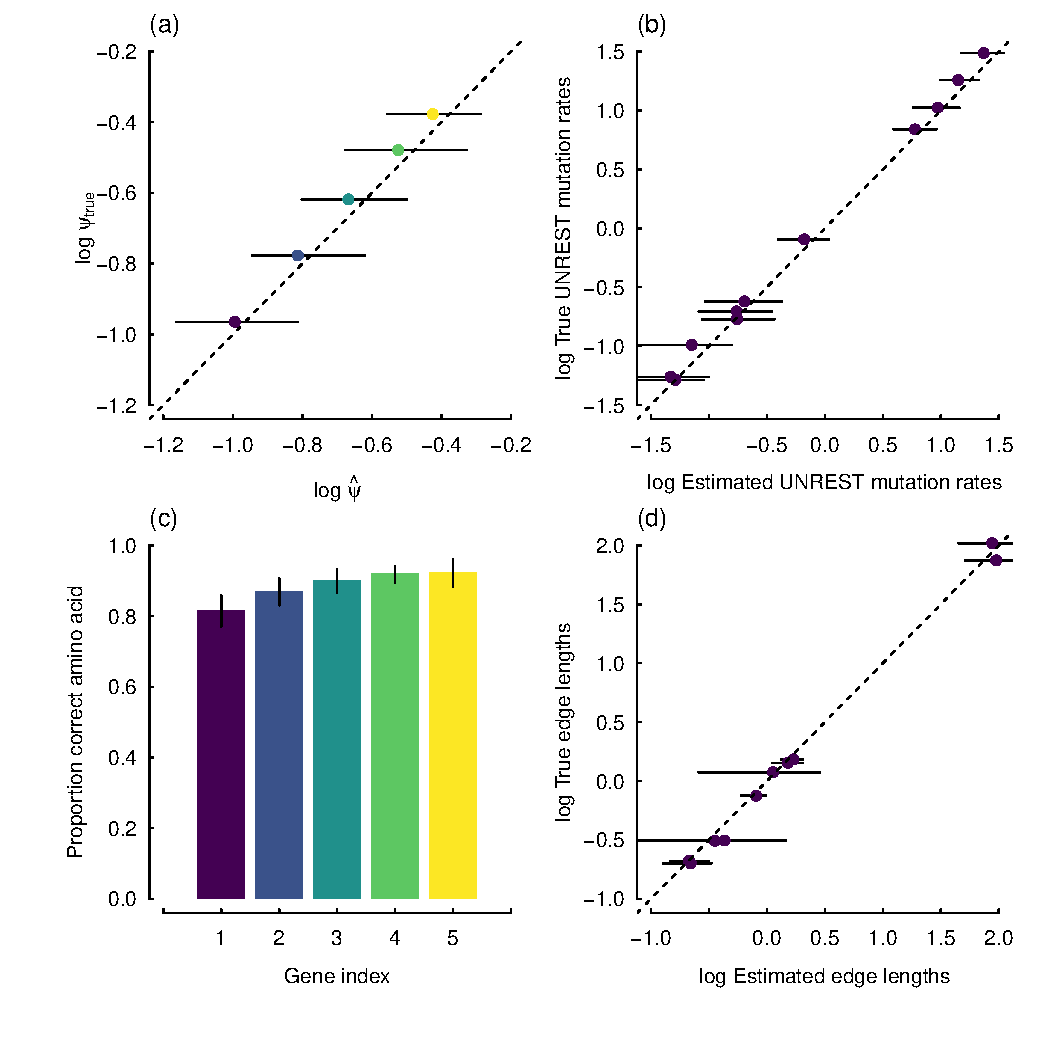
\includegraphics[width=0.9\linewidth]{FIGURE_1_5genes_All_UNREST_WITHGAMMA.pdf}
  \caption{Summary of a 5-gene simulation for a SelAC model where we assume $\alphag = \infty$, and thus, no site-specific sensitivity in the generating model.
    The `known' parameters were based on fitting the SelAC model to the 106 gene data set and phylogeny of \citet{RokasEtAl2003}, with gene choice being based on five evenly spaced points along the rank order of the gene specific composite parameter $\psiprime_g$.
                The points and associated uncertainty in the estimates of the gene-specific average protein synthesis rate, or $\psi$ (calculated from $\psiprime$)(a), nucleotide mutation rates under the UNREST model (b), proportion of correct optimal amino acids for a given gene (c), and estimates of the individual edge lengths are based the mean and 2.5\% and 97.5\% quantiles across all 50 simulated datasets (d).
                Gene index on the x-axis refers to the arbitrary number assigned to the simulated gene.
    }
  \label{fig:SelacWithGSimRes}
\end{figure}


\begin{figure}[H]
  \centering
  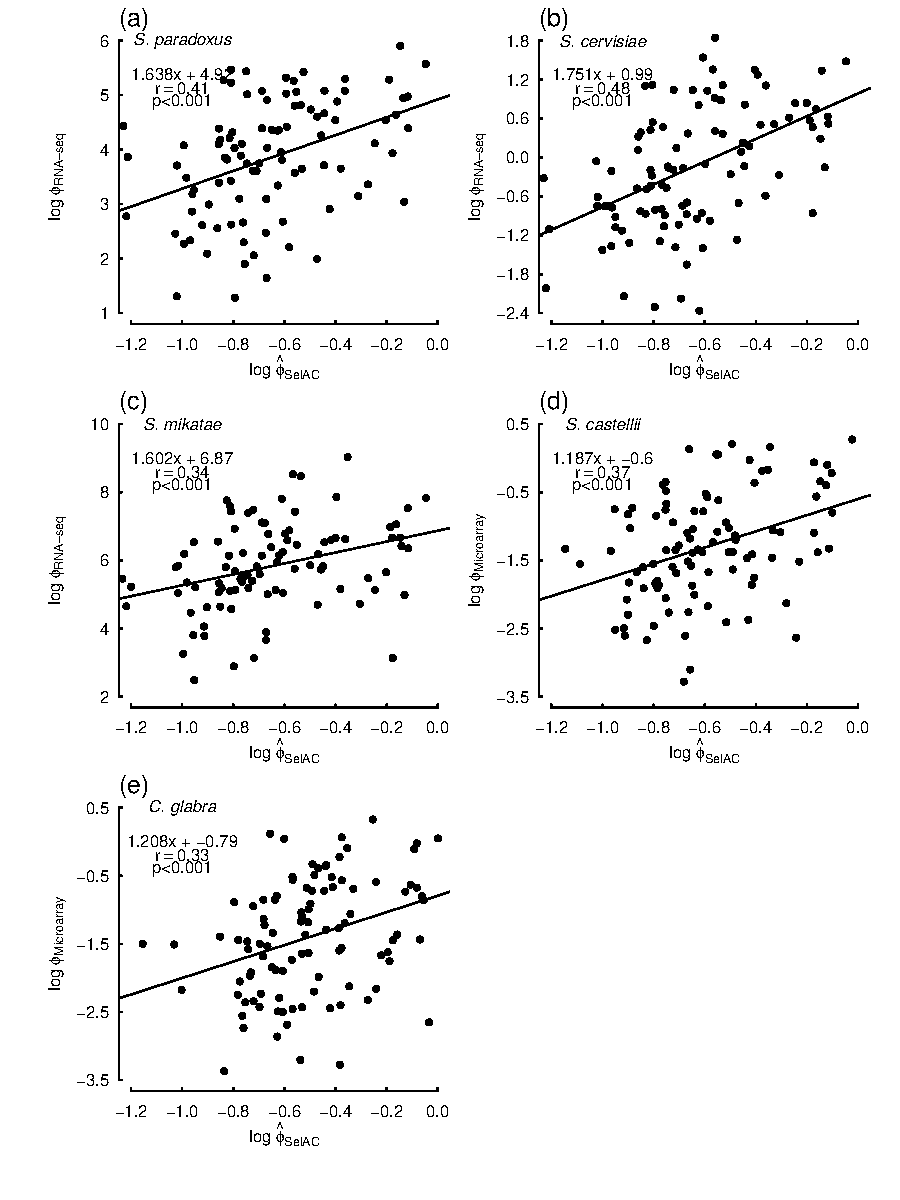
\includegraphics[width=0.9\linewidth]{FIGURE_2_SelACwG_vs_Empirical_by_spp_ALLspp.pdf}
  \caption{Comparisons between estimates of average protein translation rate $\phihat$ obtained from \selacplusgamma and direct measurements of expression for individual yeast taxa across the 100 selected genes from \citet{SalichosAndRokas2013} measured during log-growth phase.
        Estimates of $\phihat$ were generated by dividing the composite term $\psiprime$ by \Funcaveci.
        Gene expression was measured using either RNA-Seq (a)-(c) or microarray (d)-(e).
        The equations in the upper left hand corner of each panel represent the regression fit and the Pearson correlation coefficient $r$.
  }
  \label{fig:PhivsEmpirical}
\end{figure}


\begin{figure}[H]
  \centering
  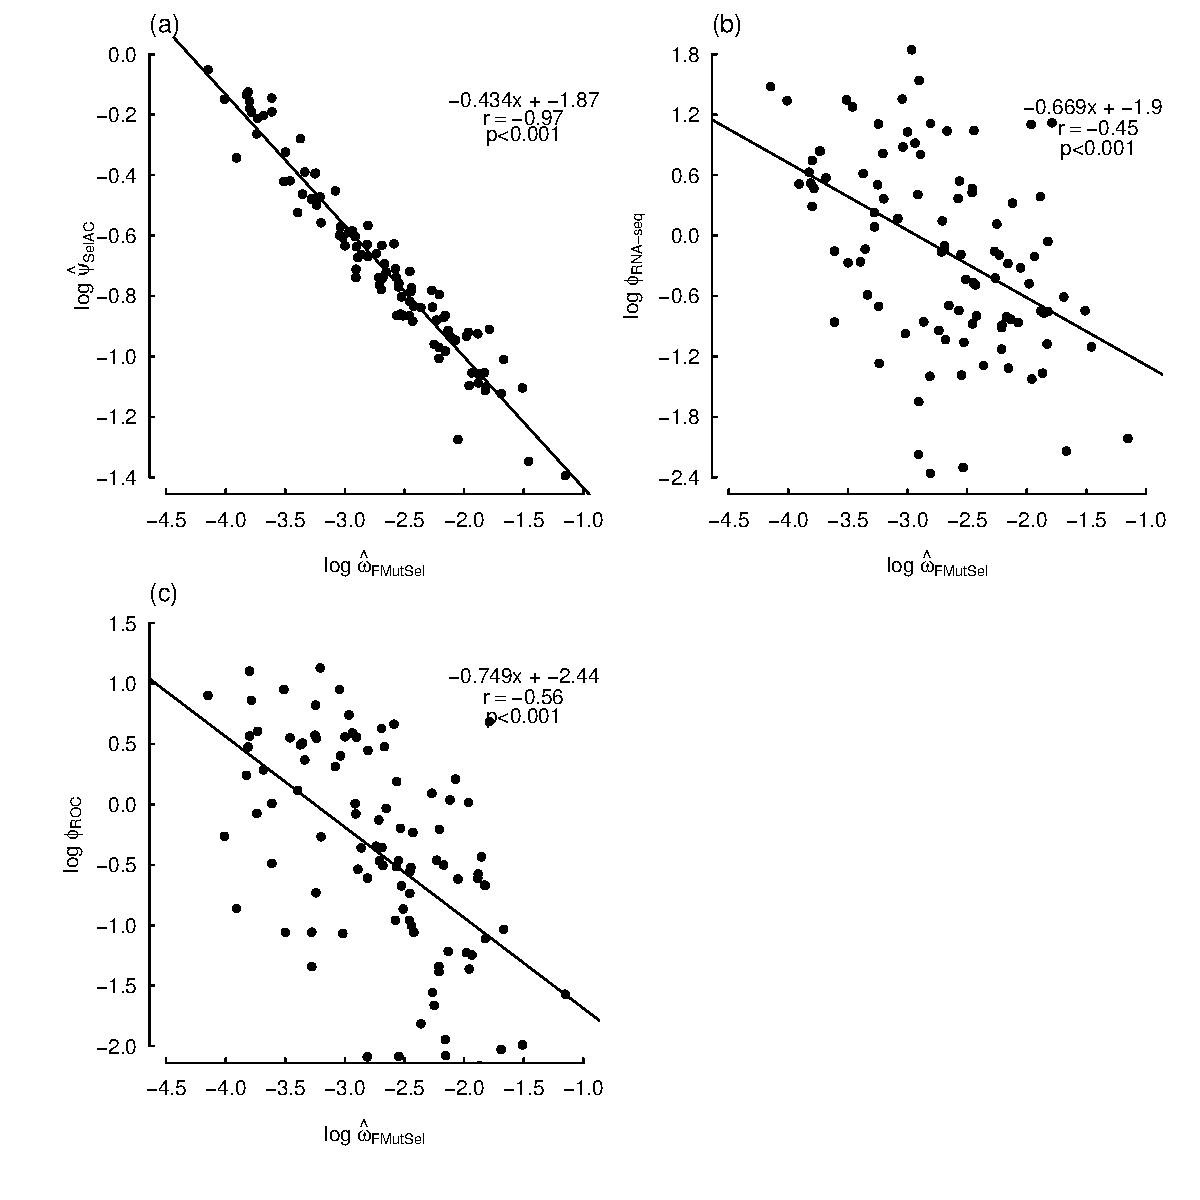
\includegraphics[width=0.9\linewidth]{FIGURE_3_MutSelOmega_vs_Us_ROC_Scer_only.pdf}
  \caption{Comparisons between $\omega_{\text{FMutSel}}$, which is the nonsynonymous/synonymous mutation ratio in FMutSel, \selacplusgamma estimates of protein functionality production rates $\psihat$ (a), RNA-Seq based measurements of mRNA abundance $\phi_{\text{RNA-seq}}$ (b), and ROC-SEMPPER's estimates of protein translation rates $\phi_{\text{ROC}}$, which are based solely on \emph{S.~cerevisiae}'s patterns of codon usage bias (c), for \emph{S.~cerevisiae} across the 100 selected genes from \citet{SalichosAndRokas2013}.
    As in Figure \ref{fig:PhivsEmpirical}, the equations in the upper right hand corner of each panel provide the regression fit and correlation coefficient.
}
  \label{fig:OmegavsPsi}
\end{figure}


\begin{figure}[H]
  \centering
  \includegraphics[width=0.9\linewidth]{FIGURE_4_Inferred_Tree_AND_Model_Adequacy.pdf}
  \caption{(a) Maximum likelihood estimates of branch lengths under \selacplusgamma for 100 selected genes from \citet{SalichosAndRokas2013}.
    Tests of model adequacy for \emph{S.~cerevisiae} (b) and \emph{S.~castellii} (c) indicated that, when these taxa are removed from the tree, and their sequences are simulated, the parameters of \selacplusgamma exhibit functionality \Funcaobsvec that is far closer to the observed (dashed black line) than data sets produced from parameters of either FMutSel or GTR + $\Gamma$.
}
  \label{fig:TreeAndAdequacy}
\end{figure}



\ifthenelse{1=1}{ %include supporting materials}
\clearpage



\appendix

%%% commands for getting SM pages and figures labeled with S
%% different than with other .cls
\setcounter{section}{19} %appendix environment set in .cls file.  Set this to 19 to get an 'S' for figures
\setcounter{page}{1}
\renewcommand{\thepage}{S\arabic{page}} %this works

\section{Supporting Materials}
Supporting Materials for \emph{Population Genetics Based Phylogenetics Under Stabilizing Selection for an Optimal Amino Acid Sequence: A Nested Modeling Approach} \ by Beaulieu \emph{et al.}~(In Review).

\subsection{Comparisons of SelAC gene expression estimates with empirical measurements}
In our model, the parameter $\phi$ measures the realized average protein synthesis rate of a gene.
We compared our estimates of $\phi$ to two separate measures of gene expression, one empirical (Figure \ref{fig:PhivsROC}), and one model-based prediction that does not account for shared ancestry, for individual yeast taxa across the same set of genes.
Our estimates of $\phi$ are positively correlated with both measures, which are also reasonably well correlated with each other (Figure \ref{fig:PhivsEmpirical} - \ref{fig:ROCvsEmpirical})
On the whole, these comparisons indicate not only a high degree of consistency among all three measures, but also, importantly, that estimates of $\phi$ obtained from SelAC provide real biological insight into the expression level of a gene.

\vfill

\begin{figure}%[H]
  \centering
  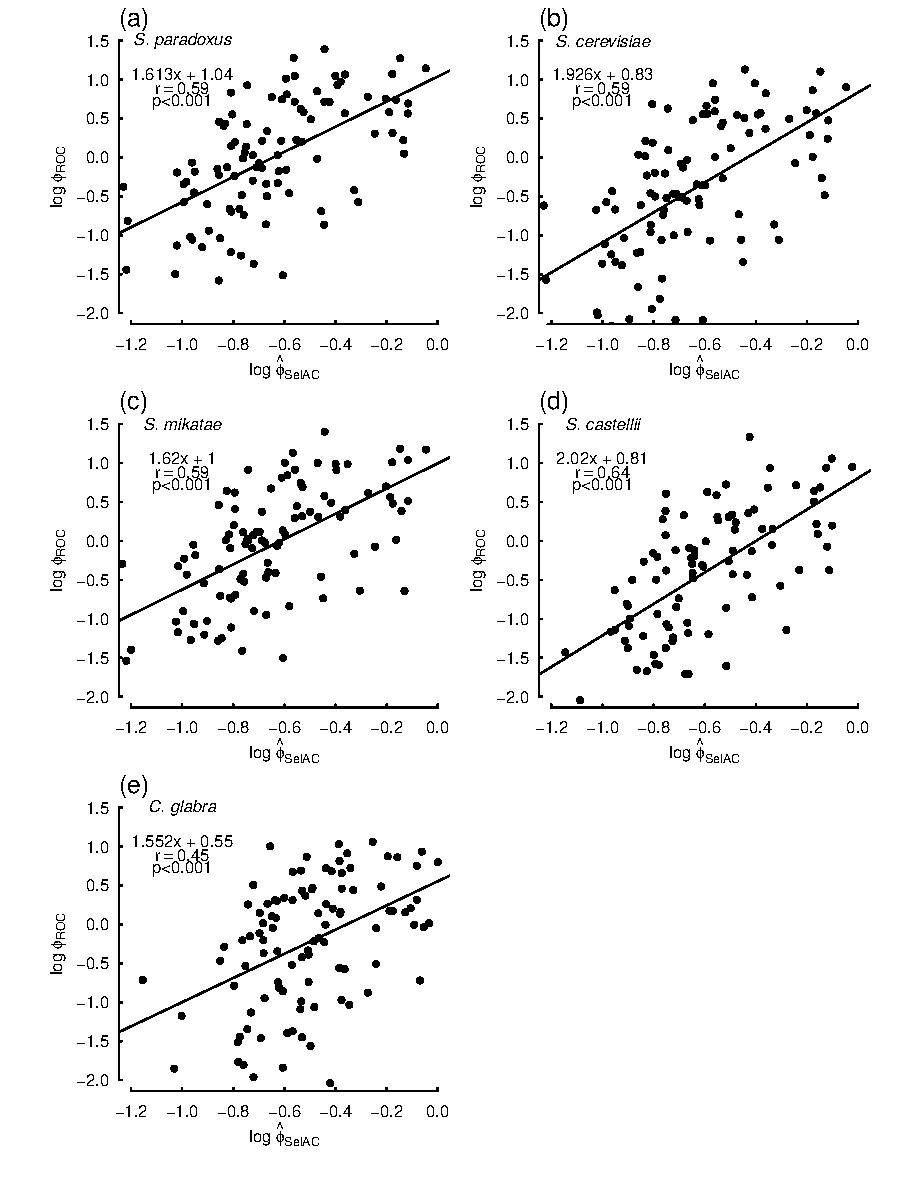
\includegraphics[width=0.9\linewidth]{FIGURE_S1_SelACwG_vs_ROC_by_spp_ALLspp.pdf}
  \caption{Comparisons between estimates of $\phi$ obtained from \selacplusgamma and the predicted gene expression from the ROC SEMPER model \citep{GilchristEtAl2015} for individual yeast taxa across the 100 selected genes from \citet{SalichosAndRokas2013}.
        As with figures in the main text, estimates of $\phi$ were obtained by solving for $\psi$ based on estimates of $\psiprime$, and then dividing by \Funcaveci.
                The equations in the upper left hand corner of each panel represent the regression fit and correlation coefficient.
  }
  \label{fig:PhivsROC}
\end{figure}


\begin{figure}[H]
  \centering
  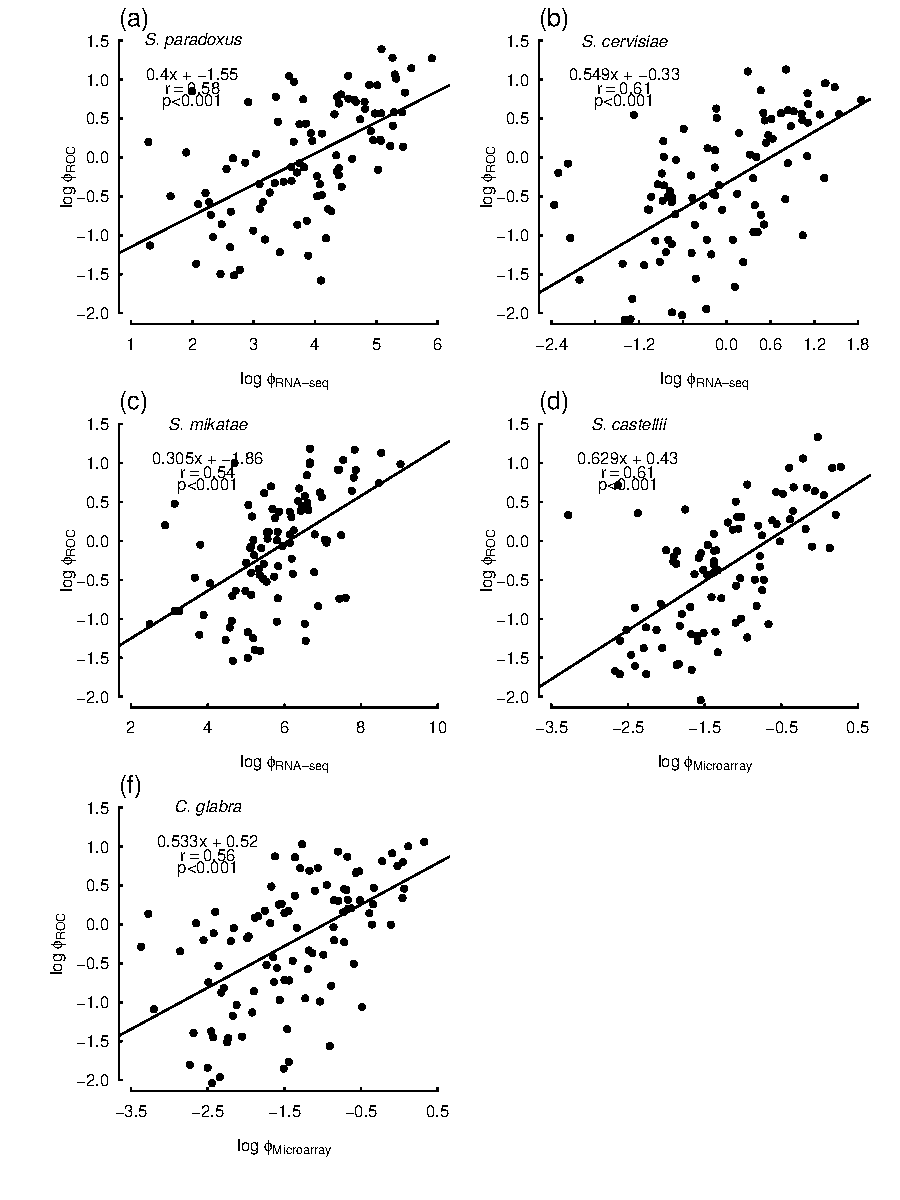
\includegraphics[width=0.9\linewidth]{FIGURE_S2_Empirical_vs_ROC_by_spp_ALLspp.pdf}
  \caption{Comparisons of predicted gene expression from the ROC SEMPER model (\citet{GilchristEtAl2015}) and direct measurements of expression from RNA-Seq or microarray data for individual yeast taxa across the 100 selected genes from \citet{SalichosAndRokas2013}.
        The equations in the upper left hand corner of each panel represent the regression fit and correlation coefficient.
}
  \label{fig:ROCvsEmpirical}
\end{figure}


\section*{Table}
\newcommand{\tableLabelRow}{Rank&Model&$-\ln(\Lik)$&df&AIC&AICc&\DeltaAIC&\DeltaAICc\\ \hline}
%\begin{table}
\begin{longtable}{rlrrrrrr}
\caption{Comparison of \selac to 163 other phylogenetic models to 100 selected genes from 6 yeast taxa \citet{SalichosAndRokas2013} using negative log likelihood ($-ln(\Lik)$), AIC, and AICc values.
See Table \ref{table:modelFits} for more details
Models of Rank 1-4, 88, and 166 were fitted using the \selac software package.  All remaining models were fitted using IQTree \citep{IQTree}.}\label{table:modelFitsAll}\\
%formatting info
\tableLabelRow 
\endfirsthead  %end heading for table on first page
\multicolumn{8}{c}%
{\tablename\ \thetable\ -- \textit{Continued from previous page}} \\
\hline
\tableLabelRow
\endhead %end heading for table on remaining pages
\hline \multicolumn{8}{r}{\textit{Continued on next page}} \\
\endfoot %footer for everything but last page
\hline
\endlastfoot  %footer for last page
1&\selacplusgamma&453,621&50,005&1,007,252&1,027,314&0&0\\
2&\selac&464,115&50,004&1,028,238&1,050,286&20,986&22,972\\
3&\selacmajplusgamma&465,302&50,005&1,056,613&1,076,674&49,361&49,360\\
4&FMutSel&597,141&178&1,194,637&1,194,638&187,385&167,324\\
5&KOSI07+F+R10&598,031&87&1,196,235&1,196,236&188,983&168,922\\
6&KOSI07+F+R9&598,326&85&1,196,822&1,196,822&189,570&169,508\\
7&KOSI07+F+R8&598,609&83&1,197,383&1,197,384&190,131&170,070\\
8&KOSI07+F+R7&598,940&81&1,198,041&1,198,041&190,789&170,727\\
9&GY+F+R5&599,010&79&1,198,178&1,198,179&190,926&170,865\\
10&GY+F+R4&599,017&77&1,198,188&1,198,188&190,936&170,874\\
11&GY+F+R3&599,092&75&1,198,334&1,198,334&191,082&171,020\\
12&KOSI07+F+R6&599,337&79&1,198,832&1,198,832&191,580&171,518\\
13&GY+F+R2&599,662&73&1,199,471&1,199,471&192,219&172,157\\
14&KOSI07+F+R5&599,854&77&1,199,862&1,199,862&192,610&172,548\\
15&KOSI07+F+R4&600,572&75&1,201,293&1,201,294&194,041&173,980\\
16&GY+F+G4&600,946&72&1,202,037&1,202,037&194,785&174,723\\
17&GY+F+I+G4&600,947&73&1,202,040&1,202,040&194,788&174,726\\
18&SCHN05+F+R10&601,260&87&1,202,694&1,202,694&195,442&175,380\\
19&KOSI07+F+R3&601,538&73&1,203,222&1,203,222&195,970&175,908\\
20&SCHN05+F+R9&602,116&85&1,204,402&1,204,402&197,150&177,088\\
21&KOSI07+F+R2&603,128&71&1,206,397&1,206,397&199,145&179,083\\
22&SCHN05+F+R8&603,280&83&1,206,725&1,206,726&199,473&179,412\\
23&KOSI07+F+G4&604,152&70&1,208,444&1,208,445&201,192&181,131\\
24&KOSI07+F+I+G4&604,152&71&1,208,446&1,208,446&201,194&181,132\\
25&SCHN05+F+R7&604,739&81&1,209,639&1,209,639&202,387&182,325\\
26&KOSI07+F3X4+R9&605,979&34&1,212,026&1,212,026&204,774&184,712\\
27&MGK+F3X4+R5&606,033&28&1,212,121&1,212,121&204,869&184,807\\
28&MGK+F3X4+R4&606,037&26&1,212,127&1,212,127&204,875&184,813\\
29&MGK+F3X4+R3&606,057&24&1,212,163&1,212,163&204,911&184,849\\
30&GY+F3X4+R5&606,154&28&1,212,364&1,212,364&205,112&185,050\\
31&GY+F3X4+R6&606,153&30&1,212,365&1,212,365&205,113&185,051\\
32&GY+F3X4+R4&606,181&26&1,212,414&1,212,414&205,162&185,100\\
33&GY+F3X4+R3&606,212&24&1,212,472&1,212,472&205,220&185,158\\
34&SCHN05+F+R6&606,181&79&1,212,520&1,212,520&205,268&185,206\\
35&KOSI07+F3X4+R8&606,322&32&1,212,708&1,212,708&205,456&185,394\\
36&KOSI07+F3X4+R7&606,913&30&1,213,886&1,213,886&206,634&186,572\\
37&MGK+F3X4+R2&606,960&22&1,213,965&1,213,965&206,713&186,651\\
38&SCHN05+F3X4+R10&607,042&36&1,214,155&1,214,155&206,903&186,841\\
39&GY+F3X4+R2&607,143&22&1,214,329&1,214,329&207,077&187,015\\
40&SCHN05+F+R5&607,190&77&1,214,533&1,214,534&207,281&187,220\\
41&SCHN05+F3X4+R9&607,253&34&1,214,573&1,214,573&207,321&187,259\\
42&KOSI07+F3X4+R6&607,321&28&1,214,697&1,214,697&207,445&187,383\\
43&KOSI07+F3X4+R10&607,370&36&1,214,812&1,214,812&207,560&187,498\\
44&SCHN05+F3X4+R8&607,638&32&1,215,339&1,215,339&208,087&188,025\\
45&MGK+F3X4+G4&607,662&21&1,215,365&1,215,365&208,113&188,051\\
46&MGK+F3X4+I+G4&607,663&22&1,215,370&1,215,370&208,118&188,056\\
47&GY+F+I&607,640&72&1,215,424&1,215,424&208,172&188,110\\
48&GY+F3X4+G4&607,743&21&1,215,527&1,215,527&208,275&188,213\\
49&GY+F3X4+I+G4&607,744&22&1,215,531&1,215,531&208,279&188,217\\
50&KOSI07+F3X4+R5&607,829&26&1,215,709&1,215,709&208,457&188,395\\
51&SCHN05+F+R4&607,792&75&1,215,734&1,215,735&208,482&188,421\\
52&SCHN05+F3X4+R7&608,418&30&1,216,897&1,216,897&209,645&189,583\\
53&SCHN05+F+R3&608,416&73&1,216,977&1,216,977&209,725&189,663\\
54&KOSI07+F3X4+R4&608,554&24&1,217,156&1,217,156&209,904&189,842\\
55&GY+F&608,565&71&1,217,273&1,217,273&210,021&189,959\\
56&GY+F1X4+R6&608,839&24&1,217,726&1,217,726&210,474&190,412\\
57&GY+F1X4+R5&608,842&22&1,217,728&1,217,728&210,476&190,414\\
58&GY+F1X4+R4&608,866&20&1,217,772&1,217,772&210,520&190,458\\
59&MGK+F1X4+R5&608,879&22&1,217,802&1,217,802&210,550&190,488\\
60&MGK+F1X4+R4&608,883&20&1,217,807&1,217,807&210,555&190,493\\
61&GY+F1X4+R3&608,889&18&1,217,813&1,217,813&210,561&190,499\\
62&MGK+F1X4+R3&608,907&18&1,217,851&1,217,851&210,599&190,537\\
63&SCHN05+F+R2&609,165&71&1,218,472&1,218,472&211,220&191,158\\
64&KOSI07+F3X4+R3&609,569&22&1,219,182&1,219,182&211,930&191,868\\
65&SCHN05+F3X4+R6&609,687&28&1,219,430&1,219,430&212,178&192,116\\
66&GY+F1X4+R2&609,813&16&1,219,659&1,219,659&212,407&192,345\\
67&MGK+F1X4+R2&609,820&16&1,219,672&1,219,672&212,420&192,358\\
68&SCHN05+F+G4&610,131&70&1,220,401&1,220,401&213,149&193,087\\
69&SCHN05+F+I+G4&610,131&71&1,220,403&1,220,403&213,151&193,089\\
70&GY+F1X4+G4&610,207&15&1,220,444&1,220,444&213,192&193,130\\
71&GY+F1X4+I+G4&610,208&16&1,220,447&1,220,447&213,195&193,133\\
72&MGK+F1X4+G4&610,273&15&1,220,575&1,220,575&213,323&193,261\\
73&MGK+F1X4+I+G4&610,274&16&1,220,580&1,220,580&213,328&193,266\\
74&KOSI07+F+I&610,257&70&1,220,653&1,220,653&213,401&193,339\\
75&KOSI07+F1X4+R8&610,602&26&1,221,255&1,221,255&214,003&193,941\\
76&KOSI07+F&611,155&69&1,222,448&1,222,448&215,196&195,134\\
77&KOSI07+F1X4+R7&611,353&24&1,222,755&1,222,755&215,503&195,441\\
78&SCHN05+F3X4+R5&611,498&26&1,223,048&1,223,048&215,796&195,734\\
79&KOSI07+F1X4+R6&611,809&22&1,223,662&1,223,662&216,410&196,348\\
80&KOSI07+F3X4+R2&611,865&20&1,223,769&1,223,769&216,517&196,455\\
81&MG+F3X4+R7&612,290&31&1,224,642&1,224,642&217,390&197,328\\
82&MG+F3X4+R8&612,289&33&1,224,645&1,224,645&217,393&197,331\\
83&KOSI07+F1X4+R5&612,311&20&1,224,662&1,224,662&217,410&197,348\\
84&MG+F3X4+R6&612,313&29&1,224,683&1,224,683&217,431&197,369\\
85&MG+F3X4+R5&612,336&27&1,224,725&1,224,725&217,473&197,411\\
86&MG+F3X4+R4&612,355&25&1,224,760&1,224,760&217,508&197,446\\
87&MG+F3X4+R3&612,369&23&1,224,783&1,224,783&217,531&197,469\\
88&GY94&612,670&111&1,225,563&1,225,563&218,311&198,249\\
89&KOSI07+F3X4+G4&612,932&19&1,225,903&1,225,903&218,651&198,589\\
90&KOSI07+F3X4+I+G4&612,932&20&1,225,905&1,225,905&218,653&198,591\\
91&SCHN05+F1X4+R10&612,982&30&1,226,024&1,226,024&218,772&198,710\\
92&KOSI07+F1X4+R4&612,995&18&1,226,025&1,226,026&218,773&198,712\\
93&MG+F3X4+R2&613,159&21&1,226,360&1,226,360&219,108&199,046\\
94&MGK+F3X4+I&613,206&21&1,226,454&1,226,454&219,202&199,140\\
95&KOSI07+F1X4+R9&613,259&28&1,226,574&1,226,574&219,322&199,260\\
96&SCHN05+F1X4+R9&613,320&28&1,226,696&1,226,696&219,444&199,382\\
97&SCHN05+F3X4+R4&613,713&24&1,227,474&1,227,474&220,222&200,160\\
98&SCHN05+F1X4+R8&613,817&26&1,227,686&1,227,686&220,434&200,372\\
99&MG+F3X4+G4&613,854&20&1,227,747&1,227,747&220,495&200,433\\
100&MG+F3X4+I+G4&613,856&21&1,227,753&1,227,753&220,501&200,439\\
101&KOSI07+FU+R6&614,272&19&1,228,581&1,228,581&221,329&201,267\\
102&KOSI07+FU+R5&614,454&17&1,228,942&1,228,942&221,690&201,628\\
103&GY+F3X4+I&614,457&21&1,228,957&1,228,957&221,705&201,643\\
104&SCHN05+F1X4+R7&614,535&24&1,229,119&1,229,119&221,867&201,805\\
105&KOSI07+F1X4+R3&614,556&16&1,229,144&1,229,144&221,892&201,830\\
106&MGK+F3X4&614,642&20&1,229,325&1,229,325&222,073&202,011\\
107&KOSI07+FU+R7&614,772&21&1,229,586&1,229,586&222,334&202,272\\
108&SCHN05+F1X4+R6&615,584&22&1,231,212&1,231,212&223,960&203,898\\
109&MG+F1X4+R4&615,590&19&1,231,217&1,231,217&223,965&203,903\\
110&MG+F1X4+R3&615,596&17&1,231,225&1,231,225&223,973&203,911\\
111&MGK+F1X4+I&615,826&15&1,231,682&1,231,682&224,430&204,368\\
112&GY+F3X4&615,827&20&1,231,694&1,231,694&224,442&204,380\\
113&KOSI07+FU+R4&615,916&15&1,231,862&1,231,862&224,610&204,548\\
114&SCHN05+F3X4+R3&616,067&22&1,232,178&1,232,178&224,926&204,864\\
115&GY+F1X4+I&616,171&15&1,232,372&1,232,372&225,120&205,058\\
116&MG+F1X4+R2&616,483&15&1,232,997&1,232,997&225,745&205,683\\
117&MG+F1X4+G4&616,887&14&1,233,801&1,233,801&226,549&206,487\\
118&MG+F1X4+I+G4&616,889&15&1,233,808&1,233,808&226,556&206,494\\
119&SCHN05+F1X4+R5&617,068&20&1,234,176&1,234,176&226,924&206,862\\
120&KOSI07+FU+R3&617,300&13&1,234,626&1,234,626&227,374&207,312\\
121&MGK+F1X4&617,351&14&1,234,730&1,234,730&227,478&207,416\\
122&GY+F1X4&617,744&14&1,235,515&1,235,515&228,263&208,201\\
123&KOSI07+F3X4+I&618,072&19&1,236,181&1,236,182&228,929&208,868\\
124&SCHN05+F1X4+R4&618,974&18&1,237,984&1,237,984&230,732&210,670\\
125&MG+F3X4+I&619,182&20&1,238,403&1,238,403&231,151&211,089\\
126&KOSI07+F3X4&619,604&18&1,239,244&1,239,244&231,992&211,930\\
127&KOSI07+F1X4+R2&619,779&14&1,239,585&1,239,585&232,333&212,271\\
128&SCHN05+F+I&619,826&70&1,239,792&1,239,792&232,540&212,478\\
129&MG+F3X4&620,567&19&1,241,172&1,241,172&233,920&213,858\\
130&SCHN05+F&620,670&69&1,241,477&1,241,477&234,225&214,163\\
131&KOSI07+F1X4+G4&620,863&13&1,241,751&1,241,751&234,499&214,437\\
132&KOSI07+F1X4+I+G4&620,862&14&1,241,753&1,241,753&234,501&214,439\\
133&SCHN05+F1X4+R3&621,059&16&1,242,150&1,242,150&234,898&214,836\\
134&MG+F1X4+I&622,158&14&1,244,344&1,244,344&237,092&217,030\\
135&KOSI07+FU+R2&622,429&11&1,244,879&1,244,879&237,627&217,565\\
136&SCHN05+F3X4+R2&623,050&20&1,246,140&1,246,140&238,888&218,826\\
137&SCHN05+FU+R10&623,378&27&1,246,810&1,246,810&239,558&219,496\\
138&SCHN05+F1X4+R2&623,541&14&1,247,111&1,247,111&239,859&219,797\\
139&MG+F1X4&623,675&13&1,247,376&1,247,376&240,124&220,062\\
140&SCHN05+FU+R9&623,893&25&1,247,836&1,247,836&240,584&220,522\\
141&KOSI07+FU+G4&624,314&10&1,248,647&1,248,647&241,395&221,333\\
142&KOSI07+FU+I+G4&624,313&11&1,248,647&1,248,647&241,395&221,333\\
143&SCHN05+F1X4+G4&624,399&13&1,248,823&1,248,823&241,571&221,509\\
144&SCHN05+F1X4+I+G4&624,398&14&1,248,825&1,248,825&241,573&221,511\\
145&SCHN05+FU+R8&624,408&23&1,248,861&1,248,861&241,609&221,547\\
146&SCHN05+FU+R7&624,916&21&1,249,874&1,249,874&242,622&222,560\\
147&KOSI07+F1X4+I&625,424&13&1,250,875&1,250,875&243,623&223,561\\
148&SCHN05+FU+R6&625,486&19&1,251,009&1,251,009&243,757&223,695\\
149&SCHN05+FU+R5&626,269&17&1,252,572&1,252,572&245,320&225,258\\
150&SCHN05+F3X4+G4&626,387&19&1,252,812&1,252,812&245,560&225,498\\
151&SCHN05+F3X4+I+G4&626,387&20&1,252,813&1,252,813&245,561&225,499\\
152&KOSI07+F1X4&627,290&12&1,254,605&1,254,605&247,353&227,291\\
153&SCHN05+FU+R4&627,433&15&1,254,896&1,254,896&247,644&227,582\\
154&KOSI07+FU+I&627,802&10&1,255,624&1,255,624&248,372&228,310\\
155&SCHN05+FU+R3&628,994&13&1,258,014&1,258,014&250,762&230,700\\
156&KOSI07+FU&630,149&9&1,260,316&1,260,316&253,064&233,002\\
157&SCHN05+FU+R2&632,325&11&1,264,673&1,264,673&257,421&237,359\\
158&SCHN05+F3X4+I&632,477&19&1,264,991&1,264,991&257,739&237,677\\
159&SCHN05+F1X4+I&633,183&13&1,266,392&1,266,392&259,140&239,078\\
160&SCHN05+FU+G4&633,625&10&1,267,270&1,267,270&260,018&239,956\\
161&SCHN05+FU+I+G4&633,625&11&1,267,272&1,267,272&260,020&239,958\\
162&SCHN05+F3X4&633,952&18&1,267,940&1,267,940&260,688&240,626\\
163&SCHN05+F1X4&635,039&12&1,270,102&1,270,102&262,850&242,788\\
164&SCHN05+FU+I&640,485&10&1,280,991&1,280,991&273,739&253,677\\
165&SCHN05+FU&643,334&9&1,286,686&1,286,686&279,434&259,372\\
166&GTR+G&655,116&610&1,311,553&1,311,554&304,301&284,240
\end{longtable}
%\end{table}




\subsection{Simulations}
As stated in the main text, overall, the simulation results indicate that the SelAC model can reasonably recover the known values of the generating model (Figure \ref{fig:SelacNoGSimRes} - \ref{fig:SelacWithGSimRes2}).
This includes not only the parameters in \selac, but also the optimal amino acids for a given sequence as well as the estimates of the branch lengths.
Aside from the observations noted in the main text, a reviewer pointed out to us that it may also be difficult for \selac to account for changing amino-acid, which we agree may also play a role.
It has been suggested, in studies of the behavior of the gamma distribution in applications of nucleotide substitution model, that increasing the number of rate categories can often improve accuracy of the shape parameter (\citet{MayroseEtAl2005}).
Future work will address this issue.

\begin{figure}[H]
  \centering
  \includegraphics[width=0.9\linewidth]{FIGURE_S3_5genes_ALL_UNREST_Selac_NoG.pdf}
  \caption{Same figure as in Figure 1 in the main text, except the generating model does not include a site-specific sensitivity in the generating model (i.e., $\alphag = \infty$).
}
  \label{fig:SelacNoGSimRes}
\end{figure}

\begin{figure}[H]
  \centering
  \includegraphics[width=0.9\linewidth]{FIGURE_S4_5genes_alpha_beta_UNREST_Selac_NoG.pdf}
  \caption{The distribution of estimates of the Grantham weights, $\alphac$ and $\alphap$, in a SelAC model, where we assume $\alphag = \infty$, and thus no site-specific sensitivity in the generating model.
                The dashed line represents the value used in the generating model.
  }
  \label{fig:SelacNoGSimRes2}
\end{figure}


\begin{figure}[H]
  \centering
  \includegraphics[width=0.9\linewidth]{FIGURE_S5_5genes_alpha_beta_gammashape_UNREST_WITHGAMMA.pdf}
  \caption{Same figure as in Figure S4, except the generating model includes site-specific sensitivity in the generating model (i.e., $\alphag$).
                Unlike, Grantham weights, which showed no systematic bias, there is a downward bias in estimates of $\alphag$.
  }
  \label{fig:SelacWithGSimRes2}
\end{figure}



}{} %end ifthenelse

\end{document}
